%%%%%%%%%%%%%%%%%%%%%%%%%%%%%%%%%%%%%%%%%%%%%%%%%%%
%
%  New template code for TAMU Theses and Dissertations starting Fall 2012.  
%  For more info about this template or the 
%  TAMU LaTeX User's Group, see http://www.howdy.me/.
%
%  Author: Wendy Lynn Turner 
%	 Version 1.0 
%  Last updated 8/5/2012
%
%%%%%%%%%%%%%%%%%%%%%%%%%%%%%%%%%%%%%%%%%%%%%%%%%%%
%%%                           SECTION II
%%%%%%%%%%%%%%%%%%%%%%%%%%%%%%%%%%%%%%%%%%%%%%%%%%%
\chapter{\uppercase {The DGFEM Formulation of the Multigroup $S_N$ Equations}}
\label{sec::Sn}

The movement of bulk materials and particles through some medium can be described with the statistical behavior of a non-equilibrium system. Boltzmann first devised these probabilistic field equations to characterize fluid flow via driving temperature gradients \cite{encyc_physics}. His work was later extended to model general fluid flow, heat conduction, hamiltonian mechanics, quantum theory, general relativity, and radiation transport, among others. The Boltzmann Equation can be written in the general form:

\begin{equation}
\label{eq::gen_boltzmann}
\frac{\partial u}{\partial t} = \left( \frac{\partial u}{\partial t}  \right)_{force} + \left( \frac{\partial u}{\partial t}  \right)_{advec} + \left( \frac{\partial u}{\partial t}  \right)_{coll}
\end{equation}

\noindent where $u(\vec{r},\vec{p},t)$ is the transport distribution function parameterized in terms of position, $\vec{r}=(x,y,z)$, momentum, $\vec{p}=(p_x,p_y,p_z)$, and time, $t$. In simplified terms, Eq. (\ref{eq::gen_boltzmann}) can be interpreted that the time rate of the change of the distribution function, $\frac{\partial u}{\partial t}$, is equal to the sum of the change rates due to external forces, $\left( \frac{\partial u}{\partial t}  \right)_{force} $, advection of the particles, $\left( \frac{\partial u}{\partial t}  \right)_{advec}$, and particle-to-particle and particle-to-matter collisions, $\left( \frac{\partial u}{\partial t}  \right)_{coll}$ \cite{mcgraw_physics}. 

For neutral particle transport, the following assumptions \cite{duderstadt1979transport} about the behavior of the radiation particles can be utilized:

\begin{enumerate}
	\item Particles may be considered as points;
	\item Particles do not interact with other particles;
	\item Particles interact with material target atoms in a binary manner;
	\item Collisions between particles and material target atoms are instantaneous;
	\item Particles do not experience any external force fields ({\em e.g.} gravity).
\end{enumerate}

These assumptions lead to the first order form of the Boltzmann Transport Equation, which we simply call the transport equation for brevity. The remainder of the chapter is outlined as follows. Section \ref{sec::Sn_neut} provides the general form of the neutron transport equation with some variants. Section \ref{sec::Sn_MG} describes how we discretize the transport equation in energy with the multigroup methodology and Section \ref{sec::Sn_Angle} presents the angular discretization via collocation. Section \ref{sec::Sn_BC} details which boundary conditions will be employed for our work. Section \ref{sec::Sn_Spatial} will conclude our discretization procedures in the spatial domain. Section \ref{sec::Sn_Solution} will present the iterative procedures used to converge our solution space. We then present concluding remarks for the chapter in Section \ref{sec::Sn_Conclusions}.

%%%%%%%%%%%%%%%%%%%%%%%%%%%%%%%%%%%%%%%%%%%%%%%%%%%
%%%   Section - Neutron Transport Equation
\section{The Neutron Transport Equation}
\label{sec::Sn_neut}

The time-dependent neutron angular flux, $\Psi (\vec{r}, E, \vec{\Omega}, t)$, at spatial position $\vec{r}$, with energy $E$ moving in direction $\vec{\Omega}$ and at time $t$, is defined within an open, convex spatial domain $\mathcal{D}$, with boundary, $\partial \mathcal{D}$, by the general neutron transport equation:


\begin{equation}
\label{eq::Sn_transport_eq_full}
\begin{aligned}
	\frac{\partial \Psi}{\partial t} + \vec{\Omega} \cdot \vec{\nabla} \Psi (\vec{r}, E, \vec{\Omega},t)+ \sigma_t (\vec{r}, E,t) \Psi (\vec{r}, E, \vec{\Omega},t) =Q_{ext} (\vec{r}, E, \vec{\Omega},t) \\
	+ \frac{\chi (\vec{r}, E,t)}{4 \pi} \int dE' \nu \sigma_f (\vec{r}, E',t) \int d\Omega' \Psi (\vec{r}, E', \vec{\Omega}',t) \\ 
	+ \int dE' \int d\Omega' \sigma_s (E' \rightarrow E, \Omega' \rightarrow \Omega) \Psi (\vec{r}, E', \vec{\Omega}')
\end{aligned}
\end{equation}

\noindent with the following, general boundary condition:

\begin{equation}
\label{eq::Sn_transport_bc_full}
\begin{aligned}
	\Psi (\vec{r}, E, \vec{\Omega},t) = \Psi^{inc} (\vec{r}, E, \vec{\Omega},t) + \int dE' \int d\Omega' \gamma (\vec{r}, E' \rightarrow E, \vec{\Omega}' \rightarrow \vec{\Omega},t) \Psi (\vec{r}, E', \vec{\Omega}',t) \\
	\text{for } \vec{r} \in \partial \mathcal{D}^{-} \left\{   \partial \mathcal{D}, \vec{\Omega}' \cdot \vec{n} < 0  \right\}
\end{aligned} .
\end{equation}

\noindent In Eqs. (\ref{eq::Sn_transport_eq_full}) and (\ref{eq::Sn_transport_bc_full}), the physical properties of the system are defined as the following: $\sigma_t (\vec{r}, E,t)$ is the total neutron cross section, $\chi (\vec{r}, E,t)$ is the neutron fission spectrum, $\sigma_f (\vec{r}, E',t)$ is the fission cross section, $\nu (\vec{r}, E',t)$ is the average number of neutroncs emitted per fission, $\sigma_s (E' \rightarrow E, \Omega' \rightarrow \Omega,t)$ is the scattering cross section, $Q_{ext} (\vec{r}, E, \vec{\Omega},t)$ is a distributed external source, $\Psi^{inc} (\vec{r}, E, \vec{\Omega},t)$ is the incident boundary source, and $\gamma (\vec{r}, E' \rightarrow E, \vec{\Omega}' \rightarrow \vec{\Omega},t) \Psi (\vec{r}, E', \vec{\Omega}',t)$ is the boundary albedo. 

We can simplify Eq. (\ref{eq::Sn_transport_eq_full}) to:

\begin{equation}
\label{eq::Sn_transport_eq_op}
	\frac{\partial \Psi}{\partial t} + {\bf L} \Psi =  {\bf F} \Psi  + {\bf S} \Psi + {\bf Q},
\end{equation}

\noindent by dropping the dependent variable parameters and using the following operators:

\begin{equation}
\label{eq::Sn_transport_operators}
\begin{aligned}
	{\bf L} \Psi &= \vec{\Omega} \cdot \vec{\nabla} \Psi (\vec{r}, E, \vec{\Omega},t)+ \sigma_t (\vec{r}, E,t) \Psi (\vec{r}, E, \vec{\Omega},t), \\
	{\bf F} \Psi &= \frac{\chi (\vec{r}, E,t)}{4 \pi} \int dE' \nu \sigma_f (\vec{r}, E',t) \int d\Omega' \Psi (\vec{r}, E', \vec{\Omega}',t), \\
	{\bf S} \Psi &= \int dE' \int d\Omega' \sigma_s (E' \rightarrow E, \Omega' \rightarrow \Omega, t) \Psi (\vec{r}, E', \vec{\Omega}', t),  \\
	{\bf Q}       & = Q_{ext} (\vec{r}, E, \vec{\Omega},t) ,
\end{aligned}
\end{equation}

\noindent where ${\bf L}$ is the loss operator which includes total reaction and streaming, ${\bf F}$ is the fission operator, and ${\bf S}$ is the scattering operator. If we wish to analyze a transport problem at steady-state conditions, we simply drop the temporal derivative to form

\begin{equation}
\label{eq::Sn_transport_eq_op_SS}
	 {\bf L} \Psi =  {\bf F} \Psi  + {\bf S} \Psi + {\bf Q},
\end{equation}

\noindent and note that the operators of Eq. (\ref{eq::Sn_transport_operators}) no longer depend on time, $t$.

There is a special subset of transport problems that is routinely analyzed to determine the neutron behavior of a fissile system called the {\em k-eigenvalue problem}. In Eq. (\ref{eq::Sn_transport_eq_full}), $\nu (\vec{r}, E)$ acts as a multiplicative factor on the number of neutrons emitted per fission event. We replace this multiplicative factor in the following manner:

\begin{equation}
\label{eq::Sn_nubar_k}
	\nu (\vec{r}, E) \rightarrow \frac{\tilde{\nu} (\vec{r}, E)}{k},
\end{equation}

\noindent where we have introduced the eigenvalue, $k$. By also dropping the external source term, the steady-state neutron transport equation in Eq. (\ref{eq::Sn_transport_eq_op_SS}) can be rewritten into

\begin{equation}
\label{eq::Sn_transport_eq_op_keff}
	\left( {\bf L}  - {\bf S} \right) \tilde{\Psi} =  \frac{1}{k} {\bf F} \tilde{\Psi} ,
\end{equation}

\noindent where $(k, \tilde{\Psi})$ forms an appropriate eigenvalue-eigenvector pair. Of most interest is the eigenpair corresponding to the eigenvalue of largest magnitude.

We can then gain knowledge of the behavior of the neutron population in the problem by taking the full phase-space integrals of the loss operator $\int  \int \int \, {\bf L} \tilde{\Psi} \, dE \, d\Omega \, d\vec{r}$, the fission operator $\int  \int \int \, {\bf F} \tilde{\Psi} \, dE \, d\Omega \, d\vec{r}$, and the scattering operator $\int  \int \int \, {\bf S} \tilde{\Psi} \, dE \, d\Omega \, d\vec{r}$. With the appropriate eigenvector solution, $\tilde{\Psi}$, the $k$ eigenvalue then has the meaning as the multiplicative value which balances Eq. (\ref{eq::Sn_transport_eq_op_keff}) in an integral sense. This means that $k$ also has a physical meaning as well. A value $k<1$ is called subcritical and corresponds to a system whose neutron population decreases in time; a value $k=1$ is called critical and corresponds to a system whose neutron population remains constant in time; and a value $k>1$ is called supercritical and corresponds to a system whose neutron population increases in time \cite{ott1989}.


%%%%%%%%%%%%%%%%%%%%%%%%%%%%%%%%%%%%%%%%%%%%%%%%%%%
%%%   Section - Energy Discretization
\section{Energy Discretization}
\label{sec::Sn_MG}

We begin our discretization procedures by focusing on the angular flux's energy variable. An ubiquitous energy discretization procedure in the transport community is the multigroup method \cite{duderstadt1976nuclear,lewis1984computational}. The multigroup method is defined by splitting the angular flux solution into $G$ number of distinct, contiguous, and non-overlapping energy intervals called groups. We begin by restricting the full energy domain, $[0, \infty)$, into a finite domain, $E \in [E_G, E_0]$. $E_0$ corresponds to some maximum energy value and $E_G$ corresponds to some minimum energy value (typically 0). We have done this by defining $G+1$ discrete energy values that are in a monotonically continuous reverse order: $E_G < E_{G-1} <  \ldots < E_1 < E_0$. 

From this distribution of energy values, we then say that a particular energy group, $g$, corresponds to the following energy interval:

\begin{equation}
\label{eq::Sn_MG_energy_interval}
\Delta E_g \in [E_g, E_{g-1}].
\end{equation}

\noindent Figure \ref{fig::Sn_MG_energy_bands} provides a visual representation between the $G+1$ discrete energy values and the $G$ energy groups. While the order that we have prescribed may seem illogical (high-to-low) to those outside of the radiation physics community, it has been historically applied this way because radiation transport problems are iteratively solved from high energy to low energy. If the group structure is well chosen, then the transport solution can be more efficiently and easily obtained.

\begin{figure}[bht]
\centering
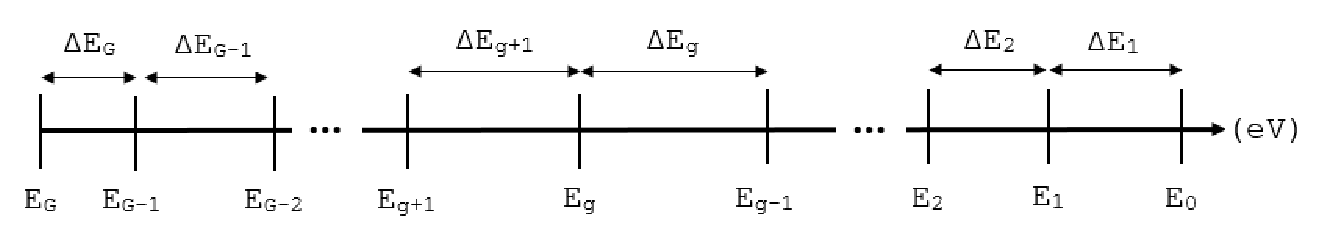
\includegraphics[width=1.00\textwidth]{figures/sec_Sn/MG_Energy_Bands.eps}
\caption{Interval structure of the multigroup methodology.}
\label{fig::Sn_MG_energy_bands}
\end{figure}

For the remainder of this energy discretization procedure, we will utilize the steady-state form of the transport equation in Eq. (\ref{eq::Sn_transport_eq_op_SS}). The time-dependent and eigenvalue forms are analagous and would be derived identically. Taking the energy interval for group $g$ as defined in Eq. (\ref{eq::Sn_MG_energy_interval}), the energy-integrated angular flux of group $g$ is

\begin{equation}
\label{eq::Sn_MG_ang_flux_g}
\Psi_g (\vec{r}, \vec{\Omega}) = \int_{E_g}^{E_{g-1}} \, \Psi (\vec{r}, E, \vec{\Omega}) \, dE .
\end{equation}

\noindent We can then use the energy-integrated angular flux to form the following coupled, $(g=1,...,G)$, discrete equations (we have dropped the spatial parameter and some of the angular parameters for further clarity):

\begin{equation}
\label{eq::Sn_MG_trans_eq}
\left(  \vec{\Omega} \cdot \vec{\nabla} + \sigma_{t,g}  \right) \Psi_g =  \sum_{g'=1}^{G} \left[ \frac{\chi_g}{4 \pi} \nu \sigma_{f,g'} \int_{4 \pi} \Psi_{g'} (\vec{\Omega}') \, d\Omega' + \int_{4 \pi} \sigma_{s}^{g' \rightarrow g} (\vec{\Omega}' , \vec{\Omega} ) \Psi_{g'} (\vec{\Omega}')  \, d\Omega'  \right] + Q_g
\end{equation}

\noindent where

\begin{equation}
\label{eq::Sn_MG_exact_condensed_terms}
\begin{aligned}
\sigma_{t,g} (\vec{r}) & \equiv \frac{\int_{E_{g}}^{E_{g-1}} \sigma_{t} (\vec{r},\vec{\Omega},E) \int_{4 \pi} \Psi (\vec{r},\vec{\Omega}, E) \, dE d\Omega}{\int_{E_{g}}^{E_{g-1}} \int_{4 \pi} \Psi (\vec{r},\vec{\Omega}, E) \, dE d\Omega}\\
\nu\sigma_{f,g} (\vec{r}) & \equiv \frac{\int_{E_{g}}^{E_{g-1}} \nu\sigma_{f} (\vec{r},E)  \int_{4 \pi} \Psi (\vec{r},\vec{\Omega}, E) \, dE d\Omega}{\int_{E_{g}}^{E_{g-1}} \int_{4 \pi} \Psi (\vec{r},\vec{\Omega}, E) \, dE d\Omega} \\
\chi_g & \equiv \int_{E_{g}}^{E_{g-1}} \chi  (\vec{r},E) \, dE \\
\sigma_{s}^{g' \rightarrow g} (\vec{r},\vec{\Omega}' , \vec{\Omega} ) & \equiv \frac{\int_{E_{g'}}^{E_{g'-1}} \left[ \int_{E_{g}}^{E_{g-1}} \sigma_s (\vec{r},E' \rightarrow E,\vec{\Omega}' , \vec{\Omega} ) \, dE \right] \Psi (\vec{r},\vec{\Omega}', E') \, dE' }{\int_{E_{g}}^{E_{g-1}}  \Psi (\vec{r},\vec{\Omega}, E) \, dE} \\
Q_g (\vec{r}, \vec{\Omega}) & \equiv \int_{E_{g}}^{E_{g-1}} Q (\vec{r}, \vec{\Omega}, E) \, dE
\end{aligned}
\end{equation}

The above equations are mathematically exact to those presented in Eqs. (\ref{eq::Sn_transport_eq_full} - \ref{eq::Sn_transport_eq_op_SS}) and we have made no approximations at this time. However, this requires full knowledge of the energy distribution of the angular flux solution at all positions in our problem domain since we weight the multigroup cross sections with this solution. This is obviously impossible since the energy distibution is part of the solution space we are trying to solve for. Instead, we now define the process to make the multigroup discretization an effective approximation method.

We first define an approximate angular flux distribution for a region $s$:

\begin{equation}
\label{eq::Sn_MG_flux_approx}
\Psi (\vec{r},\vec{\Omega}, E) =  \hat{\Psi} (\vec{r},\vec{\Omega}) f_{s} (E) ,
\end{equation}

\noindent which is a factorization of the angular flux solution into a region-dependent energy function, $f_s (E)$, and a spatially/angularly dependent function, $\hat{\Psi} (\vec{r},\vec{\Omega})$. With this approximation, we can redefine the energy-collapsed cross sections of Eq. (\ref{eq::Sn_MG_exact_condensed_terms}):

\begin{equation}
\label{eq::MG_approx_condensed_terms}
\begin{aligned}
\sigma_{t,g} (\vec{r}) & \equiv \frac{\int_{E_{g}}^{E_{g-1}} \sigma_{t} (\vec{r},E) f_{s} (E) \, dE}{\int_{E_{g}}^{E_{g-1}} f_{s} (E) \, dE} ,\\
\nu\sigma_{f,g} (\vec{r}) & \equiv \frac{\int_{E_{g}}^{E_{g-1}} \nu\sigma_{f} (\vec{r},E)  f_{s} (E) \, dE }{\int_{E_{g}}^{E_{g-1}} f_{s} (E) \, dE}, \\
\sigma_{s}^{g' \rightarrow g} (\vec{r},\vec{\Omega}' , \vec{\Omega} ) & \equiv \frac{\int_{E_{g'}}^{E_{g'-1}} \left[ \int_{E_{g}}^{E_{g-1}} \sigma_s (\vec{r},E' \rightarrow E,\vec{\Omega}' , \vec{\Omega} ) \, dE \right] f_{s} (E')\, dE' }{\int_{E_{g}}^{E_{g-1}}  f_{s} (E) \, dE} .
\end{aligned}
\end{equation}

\noindent It is noted that we do not need to redefine the fission spectrum or the distributed external sources since they are not weighted with the angular flux solution. With this energy factorization, we would expect, in general, that the approximation error will tend to zero as the number of discrete energy groups increases (thereby making the energy bins thinner). This is especially true if the group structure is chosen with many more bins in energy regions with large variations in the energy solution. For certain problems, the region-dependent energy function is well understood ({\em i.e.} almost exactly known). This means, that for these problems, we can achieve reasonable solution accuracy with only a few groups where the energy bins of the multigroup discretization are well chosen.

%%%%%%%%%%%%%%%%%%%%%%%%%%%%%%%%%%%%%%%%%%%%%%%%%%%
%%%   Section - Angle Discretization
\section{Angular Discretization}
\label{sec::Sn_Angle}

Now that we have provided the discretization of the energy variable, we next focus on the discretization of the transport problem in angle. We will do this in two stages: 1) expand the scattering source and the distributed external source in spherical harmonics and 2) collocate the angular flux at the interpolation points of the angular trial space. We will perform these discretization procedures by taking the stready-state equation presented in Eq. (\ref{eq::Sn_transport_eq_op_SS}), dropping spatial parameterization, combining the fission and external sources into a single term, and using only 1 energy group:

\begin{equation}
\label{eq::Sn_Angle_simple_trans_eq}
\vec{\Omega} \cdot \vec{\nabla} \Psi (\vec{\Omega}) + \sigma_t \Psi (\vec{\Omega}) = \int_{4 \pi}  d\Omega' \, \sigma_s ( \vec{\Omega}' \rightarrow \vec{\Omega}) \Psi (\vec{\Omega}') + Q  (\vec{\Omega}) .
\end{equation}

We first develop an approximation for the scattering term in Eq. (\ref{eq::Sn_Angle_simple_trans_eq}) by expanding the angular flux and the scattering cross section in spherical harmonics functions and Legendre polynomials, respectively. We begin by first assuming that the material is isotropic in relation to the radiation's initial direction. From this assumption, the parameterization of the scattering cross section can be written in terms of only the scattering angle, $\mu_0$,

\begin{equation}
\label{eq::Sn_scatt_xs}
\sigma_s ( \vec{\Omega}' \rightarrow \vec{\Omega}) = \frac{1}{2 \pi} \sigma_s ( \vec{\Omega}' \cdot \vec{\Omega}) = \frac{1}{2 \pi} \sigma_s ( \mu_0) , 
\end{equation}

\noindent where $\mu_0 \equiv  \vec{\Omega}' \cdot \vec{\Omega}$. With this simplification, the scattering cross section can now be expanded in an infinite series in terms of the Legendre polynomials,

\begin{equation}
\label{eq::Sn_scatt_xs_legendre}
\sigma_s ( \vec{\Omega}' \rightarrow \vec{\Omega}) = \sum\displaylimits_{p=0}^{\infty} \frac{2p + 1}{4 \pi}  \sigma_{s,p} P_p ( \mu_0) , 
\end{equation}

\noindent where $\sigma_{s,p}$ is the $p$ angular moment of the scattering cross section. These angular moments of the scattering cross section have the form:

\begin{equation}
\label{eq::Sn_scatt_xs_moments}
	\sigma_{s,p} \equiv  \int_{-1}^{1} \, d \mu_0 \, \sigma_s ( \mu_0) P_p (\mu_0)  .
\end{equation}

With the scattering cross section redefined, we can now expand the angular flux in terms of an infinite series of the spherical harmonics functions, $Y$,

\begin{equation}
\label{eq::Sn_ang_flux_sph_harm_funcs}
\Psi (\vec{\Omega}) = \frac{1}{4 \pi} \sum\displaylimits_{k=0}^{\infty} \sum\displaylimits_{n=-k}^{k} \Phi_{k,n} Y_{k,n} (\vec{\Omega})
\end{equation}

\noindent where the angular moments of the angular flux, $\Phi_{k,n}$, have the form:

\begin{equation}
\label{eq::Sn_flux_moments}
	\Phi_{k,n} \equiv \int_{4 \pi} d\Omega \, \Psi(\vec{\Omega}) \, Y_{k,n} (\vec{\Omega}).
\end{equation}

\noindent We note that the $p$ and $k$ orders of the scattering cross section and angular flux expansions, respectively, are not corresponding. We then take the scattering cross section expansion of Eq. (\ref{eq::Sn_scatt_xs_legendre}) and the angular flux expansion of Eq. (\ref{eq::Sn_ang_flux_sph_harm_funcs}), and insert them into the original scattering term of the right-hand-side of Eq. (\ref{eq::Sn_Angle_simple_trans_eq}). After significant algebra and manipulations, which we will not include here for brevity, the scattering term can be greatly simplified (the full details of this are located in Appendix \ref{sec::appendix_SN}). Eq. (\ref{eq::Sn_Angle_simple_trans_eq}) can now be written again with this alternate and simplified scattering term that is composed of the cross section and angular flux moments:

\begin{equation}
\label{eq::Sn_Angle_simple_trans_eq_w_moments_inf}
\vec{\Omega} \cdot \vec{\nabla} \Psi (\vec{\Omega}) + \sigma_t \Psi (\vec{\Omega}) = \sum_{p=0}^{\infty} \frac{2p + 1}{4 \pi} \sigma_{s,p}   \sum_{n=-p}^{p}  \Phi_{p,n}  Y_{p,n} (  \vec{\Omega} )+ Q  (\vec{\Omega}) .
\end{equation}

From the initial assumption of material isotropy (which may or not be an approximation), the scattering term of Eq. (\ref{eq::Sn_Angle_simple_trans_eq_w_moments_inf}) has introduced no approximation. Unfortunately, this form requires an infinite series expansion which we cannot use with only finite computational resources. Instead, we truncate the series at some maximum expansion order, $N_p$, which, in general, introduces an approximate form for the scattering. However, we note that if the problem scattering can be exactly captured with moments through order $N_p$, then we have introduced no approximation with this truncation. With this order of truncation, we again write the angularly continuous Eq. (\ref{eq::Sn_Angle_simple_trans_eq_w_moments_inf}), but also fold the source term into the spherical harmonics expansion,

\begin{equation}
\label{eq::Sn_Angle_simple_trans_eq_w_moments_trunc}
\vec{\Omega} \cdot \vec{\nabla} \Psi (\vec{\Omega}) + \sigma_t \Psi (\vec{\Omega}) = \sum_{p=0}^{N_p} \frac{2p + 1}{4 \pi}   \sum_{n=-p}^{p}   Y_{p,n} (  \vec{\Omega} ) \left[ \sigma_{s,p} \Phi_{p,n} + Q_{p,n}  \right] .
\end{equation}

At this point, one may wonder why we have altered the scattering operator so that it is terms of moments of the scattering cross sections and the angular flux. The reason is two-fold which will also be discussed in further detail later in this chapter. First, it greatly reduces the phase space of the scattering cross sections. With proper preprocessing, the scattering cross sections can be simplified into just their Legendre moments, instead of having to store angle-to-angle quantities ($\vec{\Omega}' \rightarrow \vec{\Omega}$). For every group-to-group combination in energy ($g' \rightarrow g$), there are only the $N_p$ moments of the scattering cross section. Secondly, the contribution of the angular flux into the scattering source with its moments can also greatly reduce the dimensional space that needs to be stored in computer memory. This will be discussed later in further detail in Section \ref{sec::Sn_Solution_Iterative}, but it simply means that we only have to store $N_{mom}$ angular flux moments for use in the scattering source. In 1 dimension, $N_{mom}$ is equal to ($N_p + 1$). In 2 dimensions, $N_{mom}$ is equal to $\frac{(N_p + 1) (N_p + 2)}{2}$. In 3 dimensions, $N_{mom}$ is equal to $(N_p + 1)^2$. For comparative purposes, we have plotted $N_{mom}$ for 1, 2, and 3 dimensions up to order 8 in Figure \ref{fig::Sn_Num_Sph_Harm_Moments}.

\begin{figure}
\centering
\includegraphics[width=0.65\textwidth]{figures/sec_Sn/Num_Sph_Harm_Moments.eps}
\caption[Number of spherical harmonics moments]{Number of spherical harmonics moments, $N_{mom}$, in 1D, 2D, and 3D as a function of the expansion order, $p$.}
\label{fig::Sn_Num_Sph_Harm_Moments}
\end{figure}

Up to this point, we have only presented the methodology to express our source terms with expansions of the spherical harmonics functions. Next, we describe the second portion of our angular discretization by deriving the standard $S_N$ equations using a collocation technique. We begin by choosing a set of $M$ distinct points and weights to form a quadrature set in angular space: $\{  \vec{\Omega}_m, w_m \}_{m=1}^M$. We will give further details about the required characteristics of this quadrature set as well as a couple of common options a little later. Using this quadrature set, we can further define a trial space for the angular flux,

\begin{equation}
\label{eq::Sn_ang_flux_basis}
\Psi (\vec{\Omega}) = \sum\displaylimits_{m=1}^{M} B_m (\vec{\Omega})  \Psi_m ,
\end{equation}

\noindent where the angular bases, $B_m$, satisfy the {\em Kronecker} property,

\begin{equation}
\label{eq::Sn_ang_basis_kroneker}
 B_j (\vec{\Omega}_m) = \delta_{j,m}, 
\end{equation}

\noindent as well as the {\em Lagrange} property,

\begin{equation}
\label{eq::Sn_ang_basis_lagrange}
\sum\displaylimits_{m=1}^{M} B_m (\vec{\Omega}_m) = 1  ,
\end{equation}

\noindent and the singular value of the angular flux along a given direction has the following notation:

\begin{equation}
\label{eq::Sn_ang_flux_identity}
\Psi_m = \Psi (\vec{\Omega}_m).
\end{equation}

Next, we substitute Eq. (\ref{eq::Sn_ang_flux_basis}) into Eq. (\ref{eq::Sn_Angle_simple_trans_eq_w_moments_trunc}), drop the external source for clarity, and collocate at the ($k=1,...,M$) interpolation (quadrature) points,

\begin{equation}
\label{eq::Sn_Angle_simple_trans_eq_w_ang_basis}
\begin{aligned}
\vec{\Omega} \cdot \vec{\nabla} \left( \sum\displaylimits_{m=1}^{M} B_m (\vec{\Omega}_k)  \Psi_m \right) + \sigma_t \left(  \sum\displaylimits_{m=1}^{M} B_m (\vec{\Omega}_k)  \Psi_m \right) \\
= \sum_{p=0}^{N_p} \frac{2p + 1}{4 \pi} \sigma_{s,p}   \sum_{n=-p}^{p}   Y_{p,n} (  \vec{\Omega} ) \left(  \sum\displaylimits_{m=1}^M \Psi_m \int_{4 \pi} d\Omega \, B_m (\vec{\Omega}_k)  \, Y_{p,n} (\vec{\Omega})  \right)  \\
k=1,...,M
\end{aligned} ,
\end{equation}

\noindent where we inserted Eq. (\ref{eq::Sn_ang_flux_basis}) into Eq. (\ref{eq::Sn_flux_moments}) to form a slightly modified form for the angular flux moments:

\begin{equation}
\label{eq::Sn_flux_mom_int_w_basis}
\Phi_{p,n} = \sum\displaylimits_{m=1}^M \Psi_m \int_{4 \pi} d\Omega \, B_m (\vec{\Omega})  \, Y_{p,n} (\vec{\Omega}).
\end{equation}

\noindent The {\em Kronecker} property of Eq. (\ref{eq::Sn_ang_basis_kroneker}), is then used at the collocation points so that Eq. (\ref{eq::Sn_Angle_simple_trans_eq_w_ang_basis}) can be simplified into the following form (where we have reintroduced the distributed source term in terms of its contribution for angle $m$):

\begin{equation}
\label{eq::Sn_trans_eq_angle_disc_FINAL}
\begin{aligned}
\vec{\Omega}_m \cdot \vec{\nabla} \Psi_{m}  + \sigma_{t}   \Psi_{m}=  \sum_{p=0}^{N_P} \frac{2p + 1}{4 \pi}  \sigma_{s,p}  \sum_{n=-p}^{p}  Y_{p,n} (  \vec{\Omega}_m )  \Phi_{p,n}  + Q_{m}  \\
m=1,...,M
\end{aligned} .
\end{equation}

Equation (\ref{eq::Sn_trans_eq_angle_disc_FINAL}) represents the transport equation that has been discretized into $M$ separate equations in angle (for 1 energy group and no spatial discretization). Up to this point, we have simply stated that there is some angular quadrature set composed of $M$ directions and weights that will satisfy some conditions of the solution, but we have not explicitly stated these conditions. For this work we will require our angular quadrature set to maintain the following properties:

\begin{enumerate}
\item The weights can sum to 1 by some normalization procedure: $\sum\displaylimits_m w_m = 1$.
\item The odd angular moments sum to $\vec{0}$: $\sum\displaylimits_m w_m \left( \vec{\Omega}_m  \right)^n =  \vec{0}$ ($n=1,3,5,...$).
\item $\sum\displaylimits_m w_m  \vec{\Omega}_m \vec{\Omega}_m = \frac{1}{3} \mathbb{I}  $, where $\mathbb{I}$ is the identity tensor.
\item The points and weights are symmetric about the primary axes in angular space. 
\item The points and weights also need to have symmetry about the problem domain boundary (this is not an issue if the domain is a rectangle in 2D or an orthogonal parallelepiped in 3D). This point is important for reflecting boundary conditions and is described in greater detail in Section \ref{sec::Sn_BC}.
\end{enumerate}

\noindent Point 4 requires some additional explanation. In 1 dimension, this corresponds to symmetry about the point 0 on the interval $[-1, 1]$. In 2 dimensions, this corresponds to quadrant-to-quadrant symmetry about the x-y primary axes of the unit circle. In 3 dimensions, this corresponds to octant-to-octant symmetry about the x-y-z primary axes of the unit sphere. 

From these properties, especially property 4, our 2D and 3D quadrature sets can be constructed in a simple and consistent manner (1D quadrature sets have different construction and our work does not include them). For both 2D and 3D problems, we can generate a subset of the quadrature points and weights on a single octant of the unit sphere, where each quadrature point in this subset has the form: $\vec{\Omega} = [\mu, \eta , \xi]$ . If we are solving a 2D problem, we would then project the quadrature points onto the $(0 < \theta < \frac{\pi}{2})$ portion of the unit circle so that they have the form: $\vec{\Omega} = [\mu, \eta ]$ (we can then view the primary octant as the primary quadrant). Once we have defined the quadrature points and weights for the primary quadrant or octant, we can then directly calculate the remainder of the quadrature set by mapping to the other quadrants or octants. Table \ref{tab::Sn_2D_octant_mapping} presents the mapping from the primary quadrant to the other 3 quadrants for 2D problems. Table \ref{tab::Sn_3D_octant_mapping} presents the mapping from the primary octant to the other 7 octants for 3D problems. In these tables, the `1' subscript corresponds to those angles generated in the primary quadrant or octant.

\begin{table}[hbt]
\centering
\caption{2D angle mapping from the first quadrant into the other 3 quadrants.}
\begin{tabular}{|c|cc|}
	\hline
	Quadrant & $\mu$ & $\eta$ \\
	\hline
	1 & $\mu_1=\mu_1$ & $\eta_1=\eta_1$ \\
	\hline
	2 & $\mu_2=-\mu_1$ & $\eta_2=\eta_1$ \\
	\hline
	3 & $\mu_3=-\mu_1$ & $\eta_3=-\eta_1$ \\
	\hline
	4 & $\mu_4=\mu_1$ & $\eta_4=-\eta_1$ \\
	\hline
\end{tabular}
\label{tab::Sn_2D_octant_mapping}
\end{table}

\begin{table}[hbt]
\centering
\caption{3D angle mapping from the first octant into the other 7 octants.}
\begin{tabular}{|c|ccc|}
	\hline
	Octant & $\mu$ & $\eta$ & $\xi $ \\
	\hline
	1 & $\mu_1=\mu_1$ & $\eta_1=\eta_1$ & $\xi_1=\xi_1$ \\
	\hline
	2 & $\mu_2=-\mu_1$ & $\eta_2=\eta_1$ & $\xi_2=\xi_1$ \\
	\hline
	3 & $\mu_3=-\mu_1$ & $\eta_3=-\eta_1$ & $\xi_3=\xi_1$ \\
	\hline
	4 & $\mu_4=\mu_1$ & $\eta_4=-\eta_1$ & $\xi_4=\xi_1$ \\
	\hline
	5 & $\mu_5=\mu_1$ & $\eta_5=\eta_1$ & $\xi_5=-\xi_1$ \\
	\hline
	6 & $\mu_6=-\mu_1$ & $\eta_6=\eta_1$ & $\xi_6=-\xi_1$ \\
	\hline
	7 & $\mu_7=-\mu_1$ & $\eta_7=-\eta_1$ & $\xi_7=-\xi_1$ \\
	\hline
	8 & $\mu_8=\mu_1$ & $\eta_8=-\eta_1$ & $\xi_8=-\xi_1$ \\
	\hline
\end{tabular}
\label{tab::Sn_3D_octant_mapping}
\end{table}

We conclude our discussion of angular discretizations by presenting two common angular quadrature sets that will be employed in this dissertation work. Section \ref{sec::Sn_Angle_LS} presents the Level Symmetric (LS) quadrature set and Section \ref{sec::Sn_Angle_PGLC} presents the Product Gauss-Legendre-Chebyshev (PGLC) quadrature set. Both of these quadrature sets can be formed from the procedure outlined before: form the primary octant and then map appropriately.

%%%%%%%%%%%%%%%%%%%%%%%%%%%%%%%%%%%%%%%%%%%%%%%%%%%
%%%   SubSection - Level-Symmetric
\subsection{Level Symmetric Quadrature Set}
\label{sec::Sn_Angle_LS}

The first quadrature set we present is the common Level Symmetric set that has had extensive use in the radiation transport community \cite{lewis1984computational,carlson1968computing}. Its defining characteristic is the restriction that it is rotationally symmetric (invariant) about all three axes of the primary octant. This leads to a two-fold additional set of restrictions: 1) once the location of the first ordinate is selected, then all other ordinates are known; and 2) the weights can become negative. This negativity of the weights can be problematic and lead to unphysical solutions if the angular flux is not sufficiently smooth.

\begin{figure}
\centering
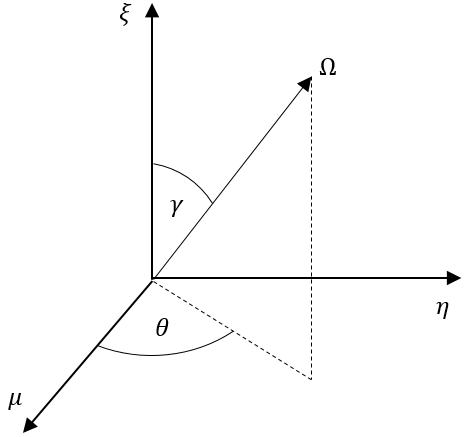
\includegraphics[width=0.45\textwidth]{figures/sec_Sn/Ang_Quad_Coord_Sys.png}
\caption[Angular Coordinate System]{Angular coordinate system for the direction $\vec{\Omega}$.}
\label{fig::Ang_Coord_Sys}
\end{figure}

We begin our description of the LS quadrature by analyzing the 3D angular coordinate system for a particular direction, $\vec{\Omega}$, as depicted in Figure \ref{fig::Ang_Coord_Sys}. The angular direction, $\vec{\Omega} = [\vec{\Omega}_x, \vec{\Omega}_y, \vec{\Omega}_z]$, is typically described with its directional cosines: $\mu$, $\eta$, and $\xi$. These are described by the angles $\theta$ and $\gamma$ of the coordinate system, which are the azimuthal and polar angles, respectively, and allow us to give a functional form for each direction component:

\begin{equation}
\label{eq::Sn_Angle_angle_components}
\begin{aligned}
\vec{\Omega}_x =& \mu = \cos (\theta) \sin (\gamma)  =\cos (\theta)  \sqrt{1 - \xi^2}  \\
\vec{\Omega}_y =& \eta = \sin (\theta) \sin (\gamma)  =\sin (\theta)   \sqrt{1 - \xi^2}   \\
\vec{\Omega}_z =& \xi = \cos (\gamma)
\end{aligned} .
\end{equation}

\noindent The direction cosines are related and necessarily must have a Euclidean norm of 1:

\begin{equation}
\label{eq::Sn_Angle_angle_cos_relation}
\mu^2 + \eta^2 + \xi^2 = 1 .
\end{equation}


We next specify the order of the quadrature set, $N$, which we restrict to only positive even integers. Each direction cosine ($\mu$, $\eta$, and $\xi$) then contains exactly $N/2$ positive values with respect to each of the three axes. This leads to exactly $\frac{N(N+2)}{8}$ total angular directions in the primary octant. Because of the rotational invariance of the quadrature set, no ordinate axis receives preferential clustering of the nodes. This means that the index value of each ordinate is identical: 

\begin{equation}
\label{eq::Sn_Angle_LS_index_values}
\mu_i = \eta_i = \xi_i, \qquad i \in (1,N/2)
\end{equation}

As previously stated, once the location of the first ordinate, $\mu_1$, is selected, then the remaining are directly known. However, to maintain the relation of Eq. (\ref{eq::Sn_Angle_angle_cos_relation}), this first ordinate has restrictions placed on it. It must maintain a positive value: $\mu_1^2 \in (0, 1/3]$. Also, for the $S2$ set (N=2), there is exactly one direction cosine with no degrees of freedom. This requires that $\mu_1^2 = 1/3$ for the $S2$ case.

With $\mu_1$ now selected, we can consider an ordinate set [$\mu_i, \eta_j, \xi_k $], where $i+j+k = N/2 + 2$. To maintain the appropriate Euclidean norm, a recursion relation can be derived (which we will not do for brevity):

\begin{equation}
\label{eq::Sn_Angle_LS_ord_det}
\mu_i^2 = \mu_{i-1}^2 + \Delta
\end{equation}

\noindent where the spacing constant, $\Delta$, has the form:

\begin{equation}
\label{eq::Sn_Angle_LS_ord_det_constant}
 \Delta = \frac{2 (1-3 \mu_1^2)}{N-2}. 
\end{equation}

\noindent Based on this recursion form, we can see that if $\mu_1^2$ is close to 0, then the ordinates will be clustered around the poles of the primary octant. Likewise, if $\mu_1^2$ is close to $1/3$, then the ordinates will be clustered away from the poles. For this work, we choose to select values of $\mu_1$ in conformance with the $LQ_N$ quadrature set because they can exactly integrate the polynomials of the Legendre expansion of the scattering cross sections \cite{carlson1971}. We finally note that the weights of the $LQ_N$ set become negative for $N \geq 20$.

We conclude this discussion of the LS quadrature set with some examples. Figure \ref{fig::Sn_Angle_LS_Quads_3D} provides a visual depiction of the LS nodes and weights in the primary octant for varying orders. The magnitude of the weights is characterized by the relative size of the nodes. Figure \ref{fig::Sn_Angle_LS_Quads_2D} then provides the projection of the 3D LS quadrature set onto to the unit circle for various orders for use in 2D problems. We have included the full quadrature set in this image including the quadrant-to-quadrant mapping. 

\begin{figure}
\centering
	\begin{subfigure}[b]{0.48\textwidth}
		\centering
		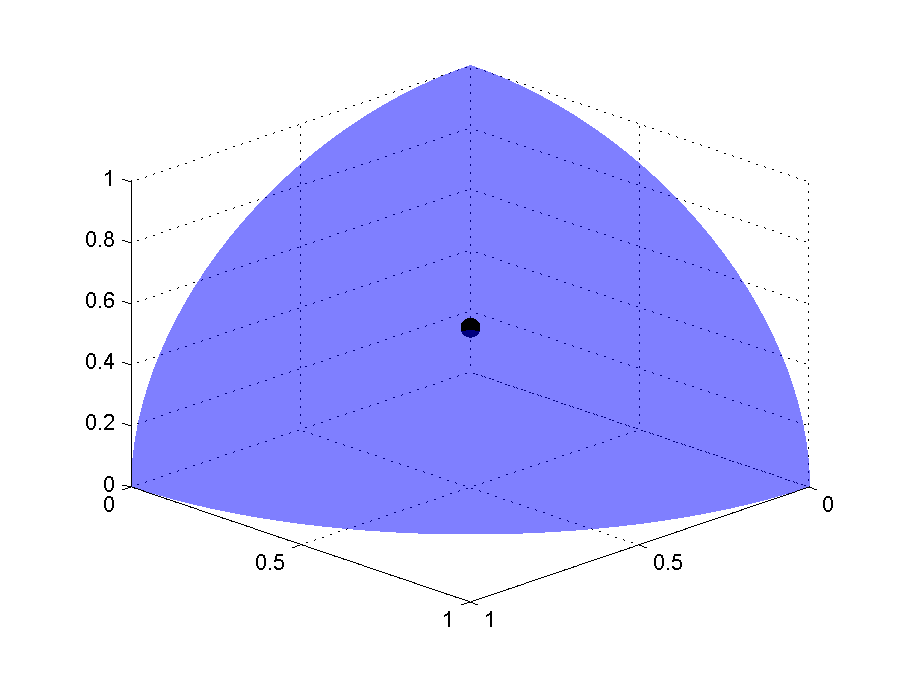
\includegraphics[width=0.92\textwidth]{figures/sec_Sn/LS2_3D.eps}
		\caption{}
	\end{subfigure}
	\hfill
	\begin{subfigure}[b]{0.48\textwidth}
		\centering
		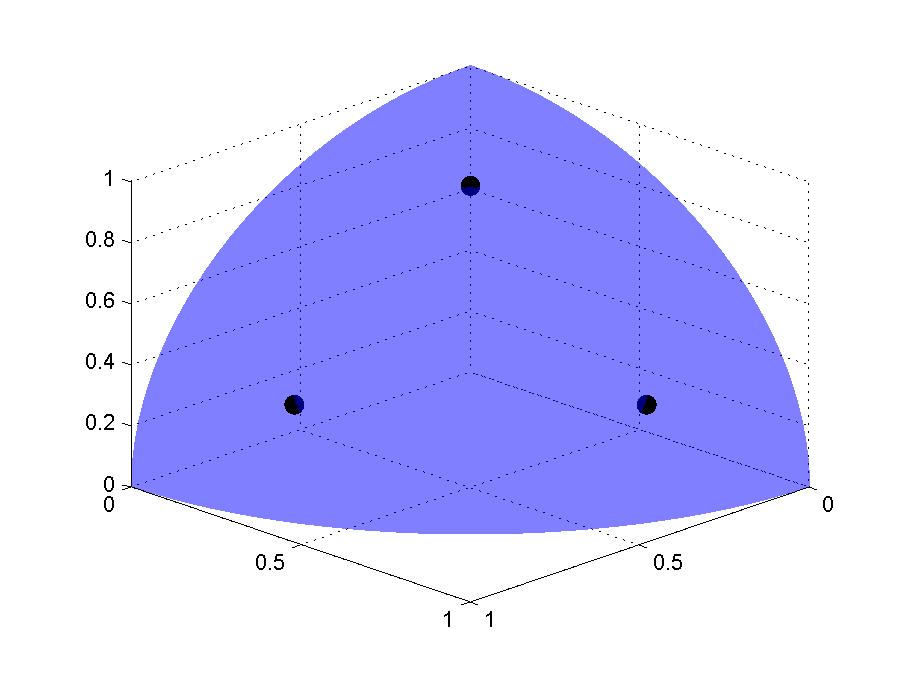
\includegraphics[width=0.92\textwidth]{figures/sec_Sn/LS4_3D.eps}
		\caption{}
	\end{subfigure}
	\vfill
	\begin{subfigure}[b]{0.48\textwidth}
		\centering
		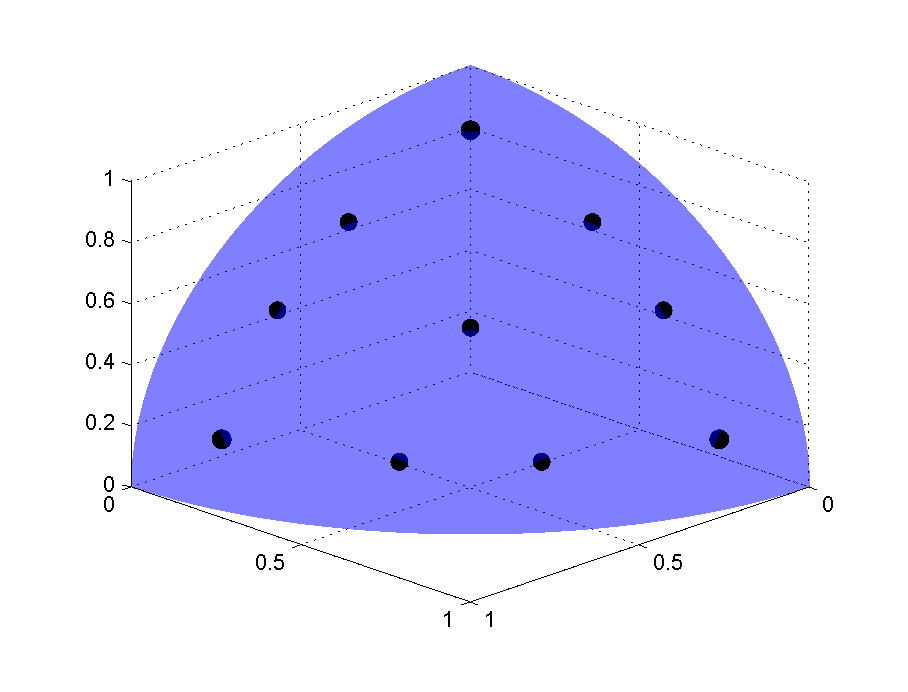
\includegraphics[width=0.92\textwidth]{figures/sec_Sn/LS8_3D.eps}
		\caption{}
	\end{subfigure}
	\hfill
	\begin{subfigure}[b]{0.48\textwidth}
		\centering
		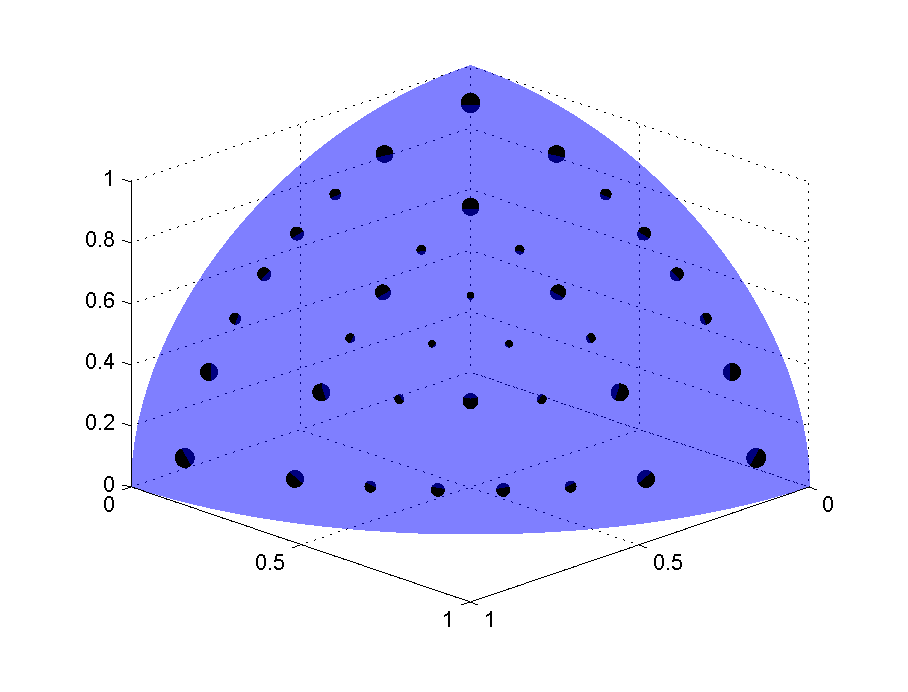
\includegraphics[width=0.92\textwidth]{figures/sec_Sn/LS16_3D.eps}
		\caption{}
	\end{subfigure}
\caption[3D Level-Symmetric angular quadrature set]{Level-Symmetric angular quadrature sets of order (a) 2, (b) 4, (c) 8, and (d) 16.}
\label{fig::Sn_Angle_LS_Quads_3D}
\end{figure}

\begin{figure}
\centering
	\begin{subfigure}[b]{0.48\textwidth}
		\centering
		\includegraphics[width=0.92\textwidth]{figures/sec_Sn/LS2_2D.eps}
		\caption{}
	\end{subfigure}
	\hfill
	\begin{subfigure}[b]{0.48\textwidth}
		\centering
		\includegraphics[width=0.92\textwidth]{figures/sec_Sn/LS4_2D.eps}
		\caption{}
	\end{subfigure}
	\vfill
	\begin{subfigure}[b]{0.48\textwidth}
		\centering
		\includegraphics[width=0.92\textwidth]{figures/sec_Sn/LS8_2D.eps}
		\caption{}
	\end{subfigure}
	\hfill
	\begin{subfigure}[b]{0.48\textwidth}
		\centering
		\includegraphics[width=0.92\textwidth]{figures/sec_Sn/LS16_2D.eps}
		\caption{}
	\end{subfigure}
\caption[2D Level-Symmetric angular quadrature set]{Projection of the 3D Level-Symmetric angular quadrature set with orders (a) 2, (b) 4, (c) 8, and (d) 16 onto the x-y space on the unit circle.}
\label{fig::Sn_Angle_LS_Quads_2D}
\end{figure}

%%%%%%%%%%%%%%%%%%%%%%%%%%%%%%%%%%%%%%%%%%%%%%%%%%%
%%%   SubSection - PGLC
\subsection{Product Gauss-Legendre-Chebyshev Quadrature Set}
\label{sec::Sn_Angle_PGLC}

The second angular quadrature set we will present is a Product Gauss-Legendre-Chebyshev (PGLC) set \cite{abu1977compatible}. It is formed by the product-wise multiplication of a Gauss-Chebyshev quadrature in the azimuthal direction and a Gauss-Legendre quadrature in the polar direction. It has the following key differences from the Level Symmetric set:

\begin{itemize}
	\item Does not have $90^o$ rotational invariance within the primary octant; however, we still maintain octant-to-octant symmetry via mapping;
	\item Has more control over the placement of the anglular directions within the primary octant;
	\item Quadrature weights are aligned with the polar level;
	\item Has strictly positive weights for all polar and azimuthal combinations.
\end{itemize}

From the listed differences, we can already discern some clear advantages and disadvantages from a fully-symmetric quadrature set like LS. If a high number of angles are required for a problem, then negative weights do not arise. This is beneficial for transport problems with significant discontinuities. Also, the quadrature directions can be preferentially distributed in the primary octant if required for a particular problem. For example, if the transport solution is smoothly varying in the polar direction and not in the azimuthal direction, then we can specify a larger number of quadrature points in the azimuthal direction, with much fewer points in the polar direction. However, this also highlights the fact that the quadrature weights are aligned with the polar level, which can lead to less accurate moment integrations for certain transport problems. 

Because the PGLC quadrature set is formed by product-wise multiplication, we simply need to specify the component nodes and weights in both the azimuthal and polar directions to fully define all ordinates in the primary octant. The azimuthal direction, $\theta$, uses the positive range of the Gauss-Chebyshev quadrature set \cite{abramowitz1966handbook}. With the azimuthal direction restricted to its positive values in the primary octant, this corresponds to the upper-right portion of the unit circle: $\theta \in [0, \pi / 2]$. If we specify $A$ azimuthal directions for our quadrature set in the primary octant, then the azimuthal nodes and weights can be directly stated as 

\begin{equation}
\label{eq::Sn_Angle_GC_quad}
\theta_m = \frac{2m - 1}{4A} \pi \qquad \text{and} \qquad w_m = \frac{\pi}{2 A} ,
\end{equation}

\noindent respectively. 

For the polar direction, a Gauss-Legendre quadrature set is used \cite{abramowitz1964handbook}. Similar to the azimuthal direction, we restrict the integration of the polar direction to its positive values: $\xi \in (0,1)$. If we specify $P$ polar directions, then the cosine of the polar nodes, $\xi$, of our quadrature set are the positive roots of the $2P$-order Legendre polynomials taken over the inveral $[-1, 1]$. In this case, we simply discard the negative roots. The corresponding Legendre weights are given by the following formula,

\begin{equation}
\label{eq::Sn_Angle_PGLC_legendre_weights}
w_n = \frac{2}{(1-\xi_n^2) (L_{2P}' (\xi_n))^2} ,
\end{equation}

\noindent where $ L_{2P}'$ is the derivative of the $2P$-order Legendre polynomial.

With the azimuthal directions specified by Eq. (\ref{eq::Sn_Angle_GC_quad}) and the polar cosines specified by the Legendre polynomial roots, any ordinate can now be determined by the definition of the angular directions in Eq. (\ref{eq::Sn_Angle_angle_components}). The ordinate weights can be specified in a similar manner. From Eqs. (\ref{eq::Sn_Angle_GC_quad}) and (\ref{eq::Sn_Angle_PGLC_legendre_weights}), any ordinate weight, $w_{m,n}$, can be calculated by the pairwise products of the azimuthal and polar weights: $w_{m,n} = w_m w_n$. This means that we can specify the integral, $F$, of some function $f (\theta, \gamma)$ over the primary octant of the unit sphere,

\begin{equation}
\label{eq::Sn_Angle_PGLC_product_weights}
F = \sum_{m=1}^{A} \sum_{n=1}^{P} w_m w_n  f(\theta_m , \gamma_n).
\end{equation}

For this dissertation, we will use the following notation to define the product nature of the PGLC quadrature points: $S_{A}^{P}$. Here, $A$ and $P$ correspond to the number of azimuthal and polar directions in the primary octant, respectively. We demonstrate this definition in Figure \ref{fig::Sn_Angle_PGLC_Quads_3D} for the primary octant with several combinations of azimuthal and polar directions. Figure \ref{fig::Sn_Angle_PGLC_Quads_2D} then presents the projections of these quadrature sets onto the unit circle for use in 2D transport problems. Again, the size of the direction marker corresponds to the relative weight of the quadrature point. One can clearly see that the weights vary on the polar levels, and all azimuthal weights on a given polar level are constant.

\begin{figure}
\centering
	\begin{subfigure}[b]{0.48\textwidth}
		\centering
		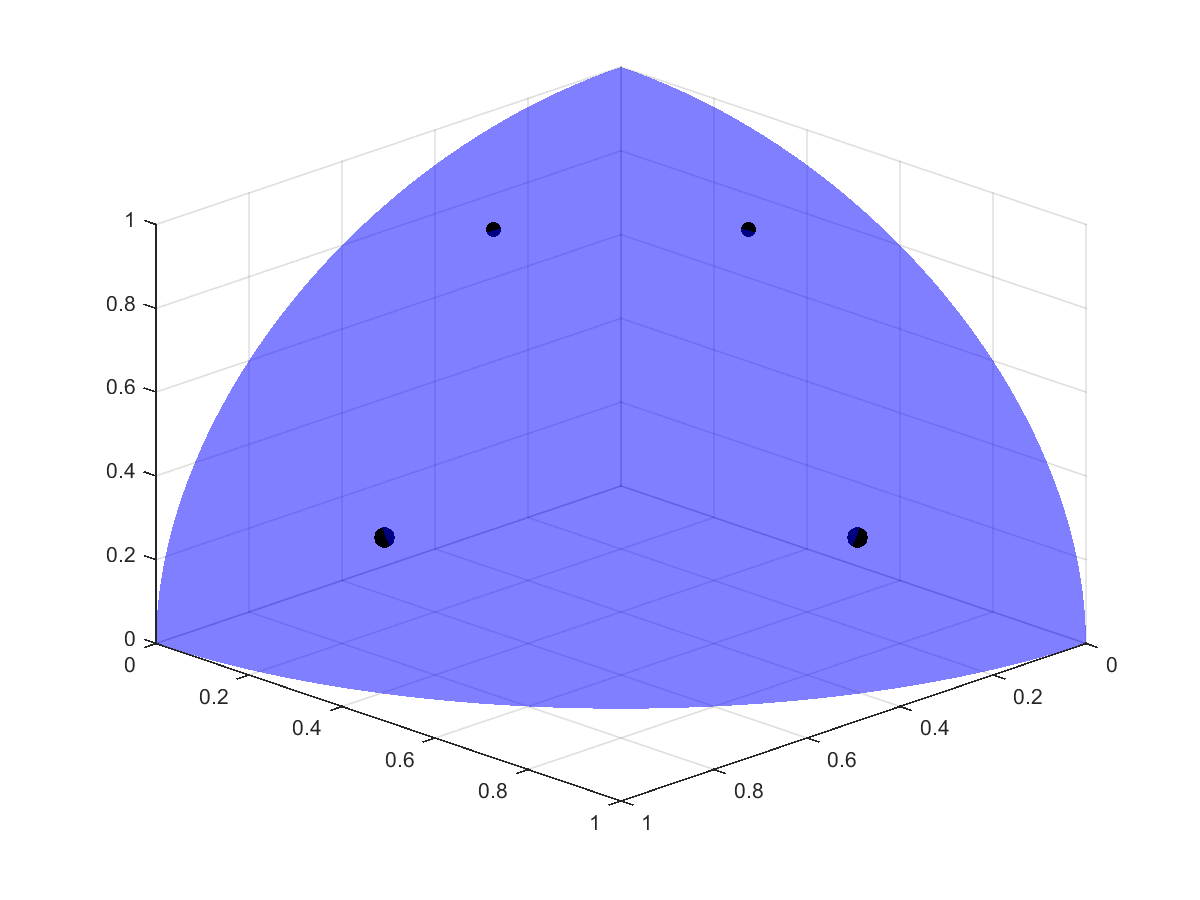
\includegraphics[width=0.92\textwidth]{figures/sec_Sn/PGLC2_2_3D.png}
		\caption{}
	\end{subfigure}
	\hfill
	\begin{subfigure}[b]{0.48\textwidth}
		\centering
		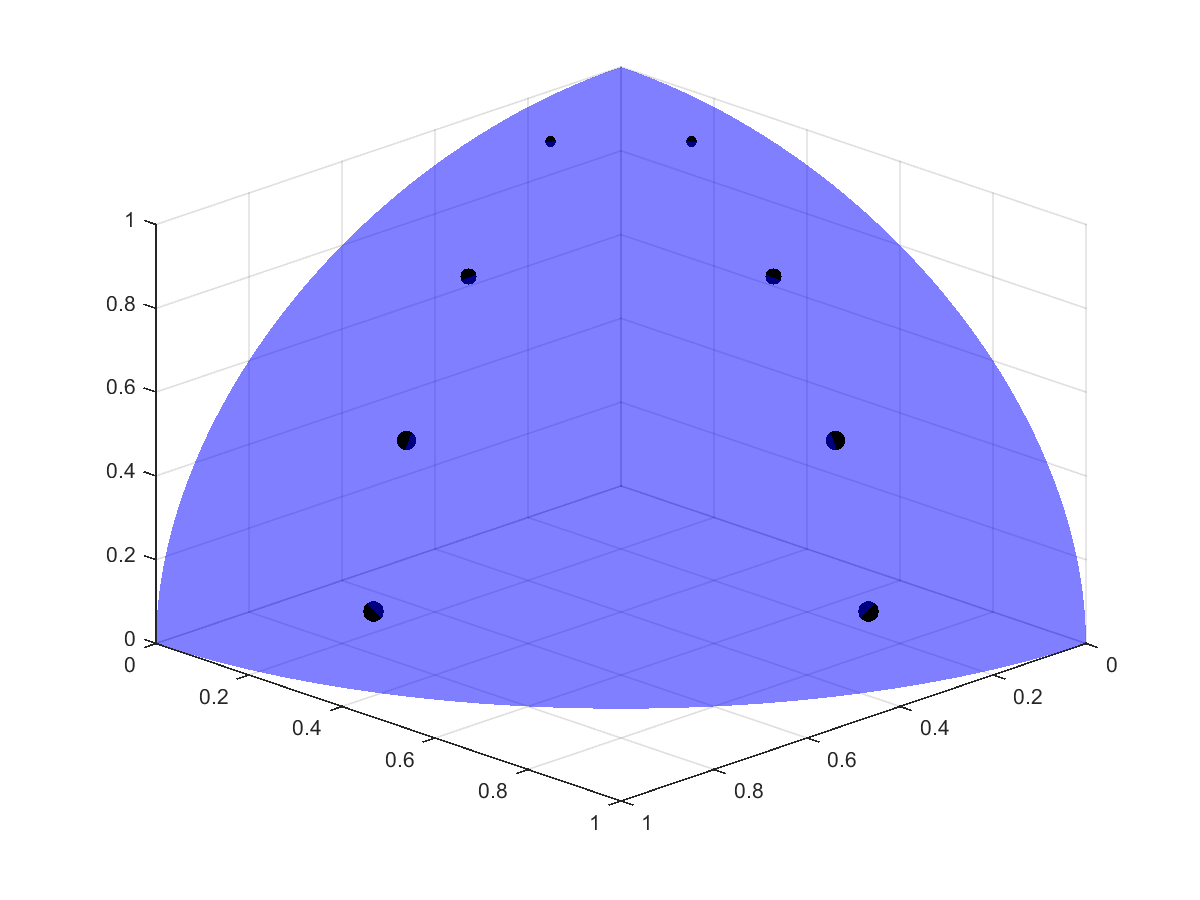
\includegraphics[width=0.92\textwidth]{figures/sec_Sn/PGLC2_4_3D.png}
		\caption{}
	\end{subfigure}
	\vfill
	\begin{subfigure}[b]{0.48\textwidth}
		\centering
		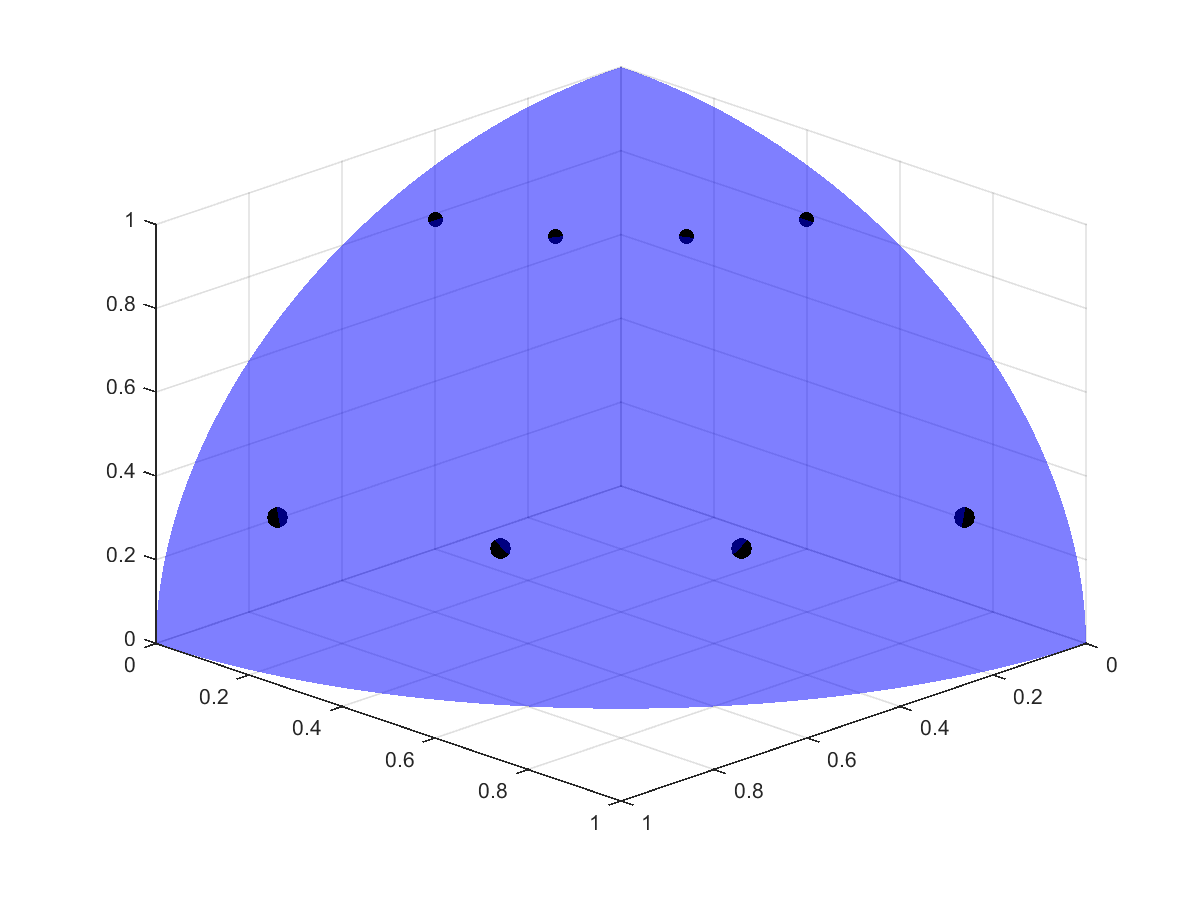
\includegraphics[width=0.92\textwidth]{figures/sec_Sn/PGLC4_2_3D.png}
		\caption{}
	\end{subfigure}
	\hfill
	\begin{subfigure}[b]{0.48\textwidth}
		\centering
		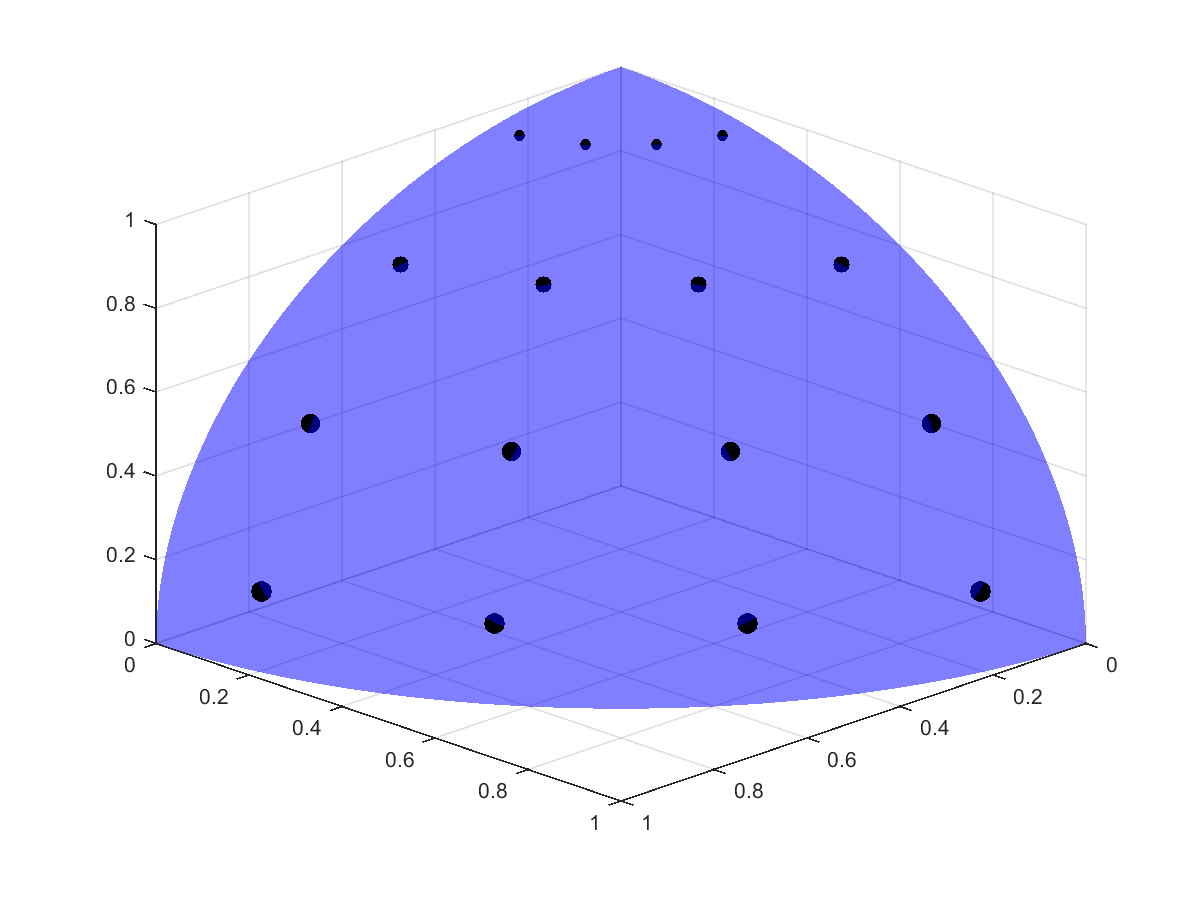
\includegraphics[width=0.92\textwidth]{figures/sec_Sn/PGLC4_4_3D.png}
		\caption{}
	\end{subfigure}
	\vfill
	\begin{subfigure}[b]{0.48\textwidth}
		\centering
		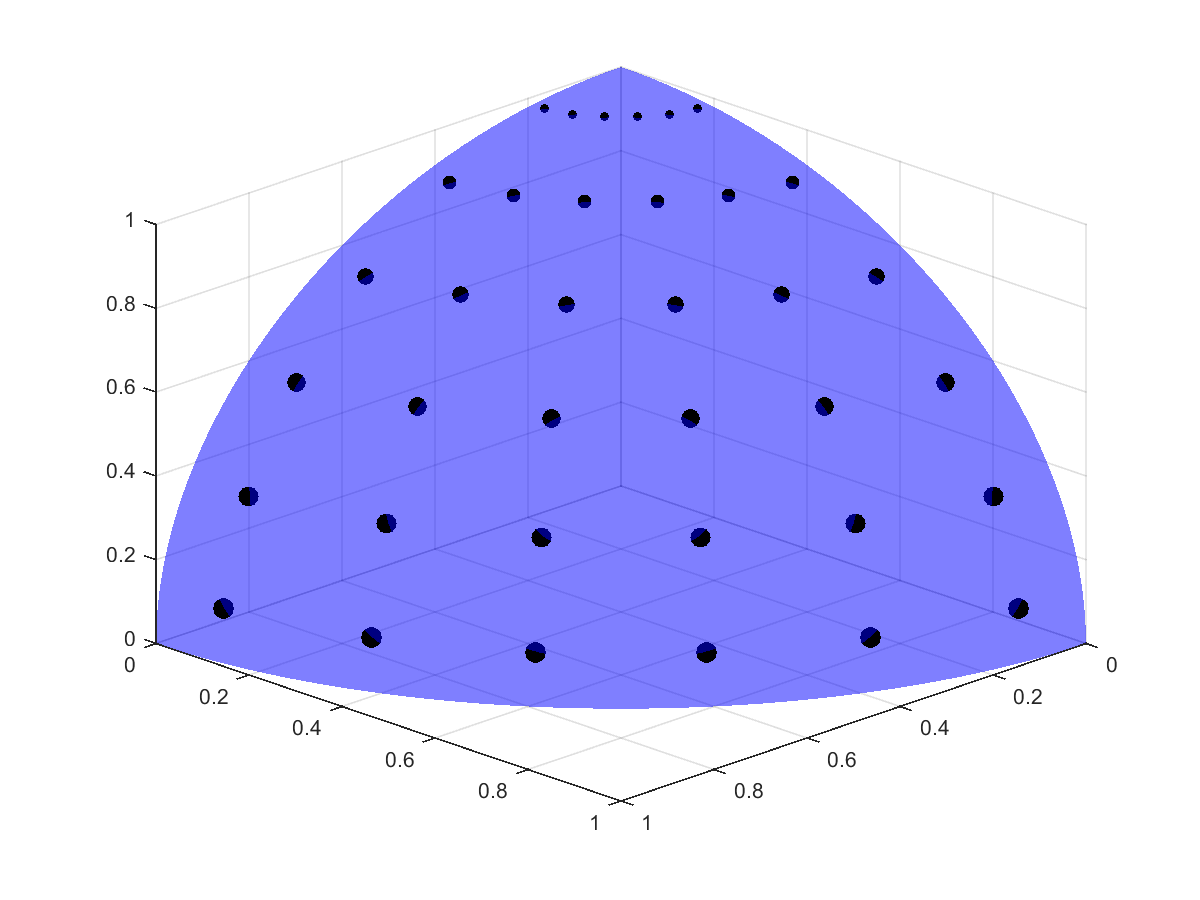
\includegraphics[width=0.92\textwidth]{figures/sec_Sn/PGLC6_6_3D.png}
		\caption{}
	\end{subfigure}
	\hfill
	\begin{subfigure}[b]{0.48\textwidth}
		\centering
		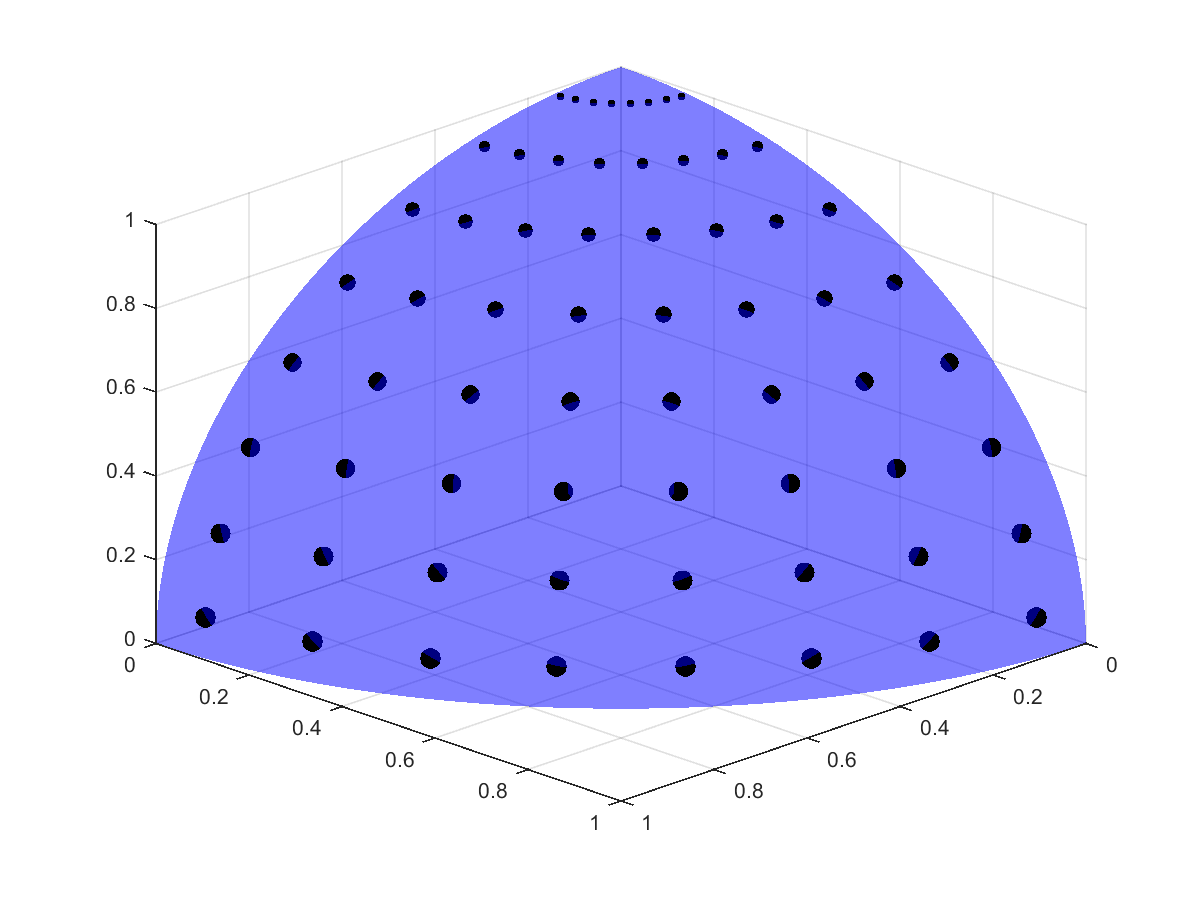
\includegraphics[width=0.92\textwidth]{figures/sec_Sn/PGLC8_8_3D.png}
		\caption{}
	\end{subfigure}
\caption[3D Product Gauss-Legendre-Chebyshev angular quadrature set]{Product Gauss-Legendre-Chebyshev angular quadrature set with orders: (a) S$_2^2$, (b) S$_2^4$, (c) S$_4^2$, (d) S$_4^4$, (e) S$_6^6$, and (f) S$_8^8$.}
\label{fig::Sn_Angle_PGLC_Quads_3D}
\end{figure}

\begin{figure}
\centering
	\begin{subfigure}[b]{0.46\textwidth}
		\centering
		\includegraphics[width=0.85\textwidth]{figures/sec_Sn/PGLC2_2_2D.eps}
		\caption{}
	\end{subfigure}
	\hfill
	\begin{subfigure}[b]{0.46\textwidth}
		\centering
		\includegraphics[width=0.85\textwidth]{figures/sec_Sn/PGLC2_4_2D.eps}
		\caption{}
	\end{subfigure}
	\vfill
	\begin{subfigure}[b]{0.46\textwidth}
		\centering
		\includegraphics[width=0.85\textwidth]{figures/sec_Sn/PGLC4_2_2D.eps}
		\caption{}
	\end{subfigure}
	\hfill
	\begin{subfigure}[b]{0.46\textwidth}
		\centering
		\includegraphics[width=0.85\textwidth]{figures/sec_Sn/PGLC4_4_2D.eps}
		\caption{}
	\end{subfigure}
	\vfill
	\begin{subfigure}[b]{0.46\textwidth}
		\centering
		\includegraphics[width=0.85\textwidth]{figures/sec_Sn/PGLC6_6_2D.eps}
		\caption{}
	\end{subfigure}
	\hfill
	\begin{subfigure}[b]{0.46\textwidth}
		\centering
		\includegraphics[width=0.85\textwidth]{figures/sec_Sn/PGLC8_8_2D.eps}
		\caption{}
	\end{subfigure}
\caption[2D Product Gauss-Legendre-Chebyshev angular quadrature set]{Projection of the 3D Product Gauss-Legendre-Chebyshev angular quadrature set with orders: (a) S$_2^2$, (b) S$_2^4$, (c) S$_4^2$, (d) S$_4^4$, (e) S$_6^6$, and (f) S$_8^8$ onto the x-y space on the unit circle.}
\label{fig::Sn_Angle_PGLC_Quads_2D}
\end{figure}

%%%%%%%%%%%%%%%%%%%%%%%%%%%%%%%%%%%%%%%%%%%%%%%%%%%
%%%   Section - Boundary Conditions
\section{Boundary Conditions}
\label{sec::Sn_BC}

Using the energy and angular discretizations presented in Sections \ref{sec::Sn_MG} and \ref{sec::Sn_Angle}, respectively, we write the standard, steady-state, multigroup $S_N$ transport equation for one angular direction, $m$, and one energy group, $g$:

\begin{equation}
\label{eq::Sn_mg_sn_trans_eq}
\begin{aligned}
	 \left( \vec{\Omega}_m \cdot \vec{\nabla}  + \sigma_{t,g}  \right)  \Psi_{m,g}= \sum_{g'=1}^{G} \sum_{p=0}^{N_P} \frac{2p + 1}{4 \pi} \sigma_{s,p}^{g' \rightarrow g}   \sum_{n=-p}^{p}  \Phi_{p,n,g'}  Y_{p,n} (  \vec{\Omega}_m )  \\
	+ \frac{\chi_g}{4 \pi} \sum_{g'=1}^{G} \nu \sigma_{f,g'} \Phi_{g'}   + Q_{m,g}
\end{aligned} , 
\end{equation}

\noindent where we have dropped the spatial parameter for clarity and is beholden to the following general, discretized boundary condition:

\begin{equation}
\label{eq::Sn_mg_sn_trans_eq_bc}
\Psi_{m,g} (\vec{r}) = \Psi^{inc}_{m,g} (\vec{r}) + \sum_{g'=1}^{G} \sum_{\vec{\Omega}_{m'} \cdot \vec{n} > 0} \gamma_{g' \rightarrow g}^{m' \rightarrow m} (\vec{r})  \Psi_{m',g'} (\vec{r})  .
\end{equation}

\noindent These $(M \text{x} G)$ number of discrete, tightly-coupled equations are currently defined as continuous in space.

For this dissertation work, we will consider only one type of boundary conditions: Dirichlet-type boundaries (also called {\em first-type boundary condition} in some physics and mathematical communities). In particular, we will only utilize incoming-incident and reflecting boundary conditions which correspond to $\vec{r} \in \partial \mathcal{D}^d$ and $\vec{r} \in \partial \mathcal{D}^r$, respectively. The full domain boundary is then the union: $\partial \mathcal{D} = \partial \mathcal{D}^d \cup \partial \mathcal{D}^r$. This leads to the boundary condition being succinctly written for one angular direction, $m$, and one energy group, $g$ as

\begin{equation}
\label{eq::Sn_simple_BC}
\Psi_{m,g} (\vec{r}) = \begin{cases}
	\Psi^{inc}_{m,g} (\vec{r}) , & \vec{r} \in \partial \mathcal{D}^d \\
	\Psi_{m',g} (\vec{r}) , & \vec{r} \in \partial \mathcal{D}^r
\end{cases}
\end{equation}

\noindent where the reflecting angle is $\vec{\Omega}_{m'} = \vec{\Omega}_{m} - 2 \left(  \vec{\Omega}_{m} \cdot \vec{n} \right) \vec{n}$ and $\vec{n}$ is oriented outward from the domain. To properly utilize the reflecting boundary condition that we have proposed, the angular quadrature set defined in Section \ref{sec::Sn_Angle} needs the following properties:

\begin{enumerate}
 	\item The reflected directions, $\vec{\Omega}_{m'}$, are also in the quadrature set for all $\vec{r} \in \partial \mathcal{D}^r$.
	\item The weights of the incident, $w_m$, and reflected, $w_{m'}$, angles must be equal.
\end{enumerate} 

\noindent For problems where the reflecting boundaries align with the $x,y,z$ axes, this will not be an issue with standard quadrature sets ({\em e.g.} level-symmetric or Gauss-Legendre-Chebyshev). However, if the reflecting boundaries do not align in this manner, then additional care must be employed in calculating appropriate angular quadrature sets.

%%%%%%%%%%%%%%%%%%%%%%%%%%%%%%%%%%%%%%%%%%%%%%%%%%%
%%%   Section - Spatial Discretization
\section{Spatial Discretization}
\label{sec::Sn_Spatial}

For the spatial discretization of the problem domain, we simplify Eq. (\ref{eq::Sn_mg_sn_trans_eq}) into a single energy group and drop the fission term (it can be lumped into the 0th order external source term and will act similarly to the total interaction term)

\begin{equation}
\label{eq::Sn_trans_eq_simple_no_energy_groups}
\vec{\Omega}_m \cdot \vec{\nabla} \Psi_{m}  + \sigma_{t}   \Psi_{m}=  \sum_{p=0}^{N_P} \frac{2p + 1}{4 \pi}    \sum_{n=-p}^{p}  Y_{p,n} (  \vec{\Omega}_m ) \left[ \sigma_{s,p}  \Phi_{p,n,}  + Q_{p,n} \right]
\end{equation}

\noindent to form $M$ ($m=1,...,M$) angularly discrete equations. We then lay down an unstructured mesh, $\mathbb{T}_h \in \mathbb{R}^{d}$, over the spatial domain, where $d$ is the dimensionality of the problem ($d=1,2,3$). This mesh consists of non-overlapping spatial elements to form a complete union over the entire spatial domain: $\mathcal{D} = \bigcup_{K \in \mathbb{T}_h} K$. To form the DGFEM set of equations \cite{ern2013theory,wareing2001discontinuous}, we consider a spatial cell $K \in \mathbb{R}^d$ which has $N_V^K$ vertices and $N_f^K$ faces. Each face of cell $K$ resides in dimension $\mathbb{R}^{d-1}$ and is formed by a connection of a subset of vertices. For a 1D problem, each face is a single point. For a 2D problem, each face is a line segment connecting two distinct points. For a 3D problem, each face is a $\mathbb{R}^2$ closed polygon (not necessarily coplanar) which may or may not be convex. An example of this interconnection between elements is given for a $\mathbb{R}^2$ problem in Figure \ref{fig::Sn_two_ref_cells} between our cell of interest, $K$, and another cell, $K'$, separated by the face $f$. We have chosen the normal direction of the face to have orientation from cell $K$ to cell $K'$ while we form the DGFEM equations for cell $K$. This means that if we were instead analyzing cell $K'$, then the face $f$ normal, $\vec{n}' $, would be opposite ({\em i.e.} $\vec{n}' = -\vec{n}$).

\begin{figure}
\centering
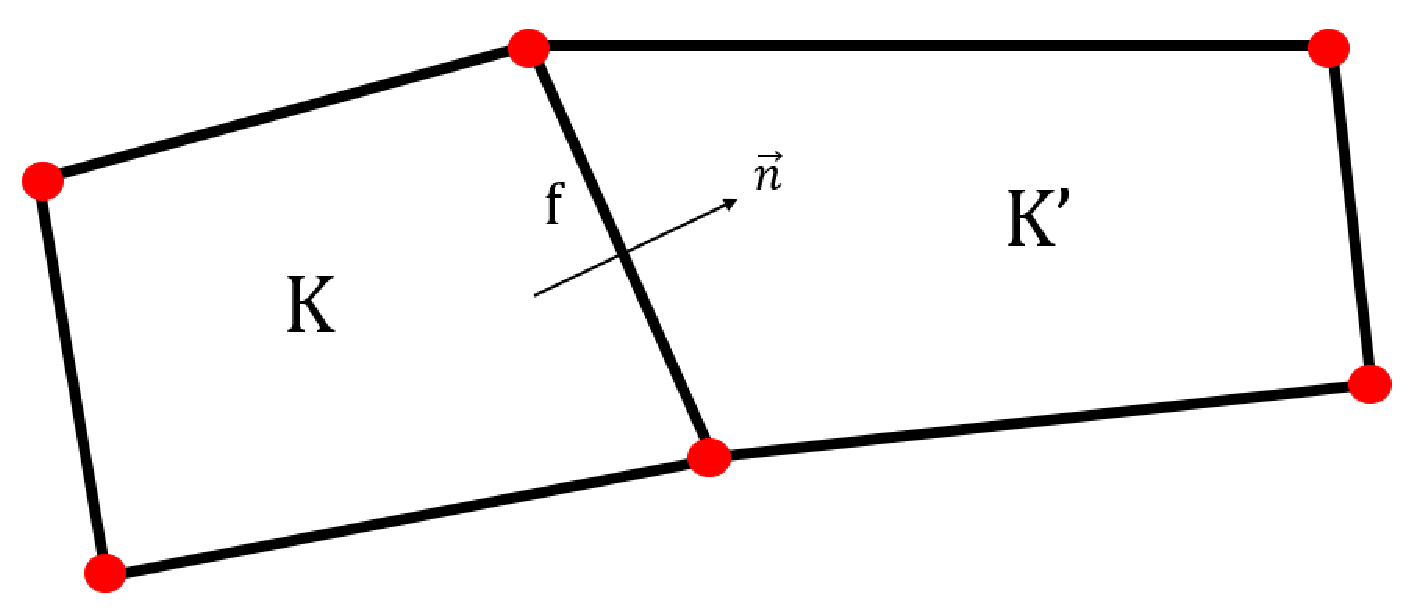
\includegraphics[width=0.7\textwidth]{figures/sec_Sn/two_cells_Rev1.eps}
\caption[Two cells of the spatial discretization]{Two cells of the spatial discretization with the connecting face, $f$, with normal direction, $\vec{n}$, oriented from cell $K$ to cell $K'$.}
\label{fig::Sn_two_ref_cells}
\end{figure}

Next, we left-multiply Eq. (\ref{eq::Sn_trans_eq_simple_no_energy_groups}) by an appropriate test function $b_m$, integrate over cell $K$, and apply Gauss' Divergence Theorem to the streaming term to obtain the Galerkin weighted-residual for cell $K$ for an angular direction $\vec{\Omega}_m$:

\begin{equation}
\label{eq::Sn_DGFEM_trans_eq_cellK}
\begin{aligned}
- \left( \vec{\Omega}_m \cdot  \vec{\nabla} b_m, \Psi_{m} \right)_{K} + \sum_{f=1}^{N_f^K} \Big< ( \vec{\Omega}_m \cdot \vec{n} ) \, b_m, \tilde{\Psi}_m  \Big>_{f}  + \Big(  \sigma_{t} b_m ,   \Psi_{m} \Big)_{K} \\
= \sum_{p=0}^{N_P} \sum_{n=-p}^{p} \frac{2p + 1}{4 \pi}  Y_{p,n} (  \vec{\Omega}_m ) \left[ \Big( \sigma_{s,p} \, b_m,  \Phi_{p,n,} \Big)_{K}  + \left(  b_m ,   Q_{p,n} \right)_{K} \right]
\end{aligned} .
\end{equation}

\noindent The cell boundary fluxes, $\tilde{\Psi}_m$, will depend on the cell boundary type and will be defined shortly. The cell boundary $\partial \mathcal{D}_K = \bigcup_{ f \in N_f^K} f$ is the closed set of the $N_f^K$ faces of the geometric cell. The inner products:

\begin{equation}
\label{eq::Sn_spatial_inner_products_cell}
 \Big( u, v \Big)_K \equiv \int_K u \, v \, d r
\end{equation} 

\noindent and

\begin{equation}
\label{eq::Sn_spatial_inner_products_face}
 \Big< u, v \Big>_f \equiv \int_f u \, v \, d s
\end{equation}

\noindent correspond to integrations over the cell and faces, respectively, where $dr \in \mathbb{R}^d$ is within the cell and $ds \in \mathbb{R}^{d-1}$ is along the cell boundary. We note that we will use this notation of the inner product for the remainder of the dissertation unless otherwise stated. We then separate the summation of the cell $K$ boundary integration terms into two different types: outflow boundaries ($\partial K^+ = \{  \vec{r} \in \partial K: \vec{n} (\vec{r}) \cdot \vec{\Omega}_m > 0 \}$) and inflow boundaries ($\partial K^- = \{  \vec{r} \in \partial K: \vec{n} (\vec{r}) \cdot \vec{\Omega}_m < 0 \}$). The inflow boundaries can further be separated into inflow from another cell: $\partial K^- \backslash \partial \mathcal{D} $; inflow from incident flux on the domain boundary: $\partial K^- \cap \partial \mathcal{D}^d $; and reflecting domain boundaries: $\partial K^- \cap \partial \mathcal{D}^r $. At this point, we note that the derivation can comprise an additional step by using Gauss' Divergence Theorem again on the streaming term. This is sometimes performed for radiation transport work so that mass matrix lumping can be performed, but we will not do so here at this time. Therefore, with the cell boundary terminology as proposed, Eq. (\ref{eq::Sn_DGFEM_trans_eq_cellK}) can be written into the following form:

\begin{equation}
\label{eq::Sn_DGFEM_trans_eq_cellK_diff_faces}
\begin{aligned}
- \left( \vec{\Omega}_m \cdot  \vec{\nabla} b_m, \Psi_{m} \right)_{K}   + \Big(  \sigma_{t} b_m ,   \Psi_{m} \Big)_{K}  \\
+  \Big< ( \vec{\Omega}_m \cdot \vec{n} ) \, b_m, \tilde{\Psi}_m  \Big>_{\partial K^+}  + \Big< ( \vec{\Omega}_m \cdot \vec{n} ) \, b_m, \tilde{\Psi}_m  \Big>_{\partial K^- \backslash \partial \mathcal{D}} \\
  + \Big< ( \vec{\Omega}_m \cdot \vec{n} ) \, b_m, \tilde{\Psi}_m  \Big>_{\partial K^- \cap \partial \mathcal{D}^d}  + \Big< ( \vec{\Omega}_m \cdot \vec{n} ) \, b_m, \tilde{\Psi}_m  \Big>_{\partial K^- \cap \partial \mathcal{D}^r}  \\
= \sum_{p=0}^{N_P} \sum_{n=-p}^{p} \frac{2p + 1}{4 \pi}  Y_{p,n} (  \vec{\Omega}_m ) \left[ \Big( \sigma_{s,p} \, b_m,  \Phi_{p,n,} \Big)_{K}  + \left(  b_m ,   Q_{p,n} \right)_{K} \right]
\end{aligned} .
\end{equation}

We can now deal with the boundary fluxes, $\tilde{\Psi}_m$, by enforcing the ubiquitously-used {\em upwind scheme}. In simple nomenclature, the upwind scheme corresponds to using the angular flux values within the cell for outflow boundaries and angular flux values outside the cell for inflow boundaries. Mathematically, the upwind scheme can succinctly be written as the following for all boundary types,

\begin{equation}
\label{eq::Sn_upwind_cases}
\tilde{\Psi}_m (\vec{r}) = \begin{cases}
\Psi_m^{-} , & \partial K^+ \\
\Psi_m^{+}, & \partial K^- \backslash \partial \mathcal{D} \\
\Psi_m^{inc}, & \partial K^- \cap \partial \mathcal{D}^d \\
\Psi_{m'}^{-}, & \partial K^- \cap \partial \mathcal{D}^r
\end{cases} ,
\end{equation}

\noindent when the following trace is applied to the angular fluxes :

\begin{equation}
\label{eq::Sn_ang_flux_trace}
\Psi_m^{\pm} (\vec{r}) \equiv \lim_{s \rightarrow 0^{\pm}} \Psi_m \Big( \vec{r} + s (\vec{\Omega}_m \cdot \vec{n}) \vec{n} \Big) .
\end{equation}

\noindent This trace has the notation, with $\vec{n}$ pointing outwards from cell $K$, of $\Psi_m^-$ corresponding to fluxes within the cell and $\Psi_m^+$ corresponding to fluxes out of the cell. Now, using the upwind scheme as previously defined, we can write our complete set of DGFEM equations for cell $K$ as

\begin{equation}
\label{eq::Sn_DGFEM_trans_eq_cellK_complete}
\begin{aligned}
-  \Big( \vec{\Omega}_m \cdot  & \vec{\nabla} b_m, \Psi_{m} \Big)_{K}   + \Big(  \sigma_{t} b_m ,   \Psi_{m} \Big)_{K} +  \Big< ( \vec{\Omega}_m \cdot \vec{n} ) \, b_m, {\Psi}_m^{-}  \Big>_{\partial K^+}  \\
  + & \Big< ( \vec{\Omega}_m \cdot \vec{n} ) \, b_m, {\Psi}_m^{+}  \Big>_{\partial K^- \backslash \partial \mathcal{D}}  + \Big< ( \vec{\Omega}_m \cdot \vec{n} ) \, b_m, {\Psi}^{-}_{m'}  \Big>_{\partial K^- \cap \partial \mathcal{D}^r}  \\
= & \sum_{p=0}^{N_P} \sum_{n=-p}^{p} \frac{2p + 1}{4 \pi}  Y_{p,n} (  \vec{\Omega}_m ) \left[ \Big( \sigma_{s,p} \, b_m,  \Phi_{p,n,} \Big)_{K}  + \left(  b_m ,   Q_{p,n} \right)_{K} \right] \\
- & \Big< ( \vec{\Omega}_m \cdot \vec{n} ) \, b_m, {\Psi}_m^{inc}  \Big>_{\partial K^- \cap \partial \mathcal{D}^d}
\end{aligned} .
\end{equation} 

\noindent We note that fluxes without the trace superscript are all within the cell. By completely defining our mathematical formulation for an arbitrary spatial cell, it is easy to see that the full set of equations to define our discretized solution space for a single angle and energy group comprises of a simple double integration loop. The full set of equations can be formed by looping over all spatial cells, $\mathcal{D} = \bigcup_{K \in \mathbb{T}_h} K$, while further looping over all faces within each cell, $\partial \mathcal{D}_K = \bigcup_{ f \in N_f^K} f$. 

%%%%%%%%%%%%%%%%%%%%%%%%%%%%%%%%%%%%%%%%%%%%%%%%%%%
%%%   SubSection - Convergence
\subsection{Convergence Rates of the DGFEM $S_N$ Equation}
\label{sec::Sn_Spatial_Convergence}

Because we seek to investigate the use of high-order spatial basis functions for the transport equation, we need to form an estimate of the spatial error based on some measure of the mesh. We do this by taking Eq. (\ref{eq::Sn_DGFEM_trans_eq_cellK_complete}), performing another integration-by-parts on the streaming term, mulitplying by the angular weight, $w_m$, and summing over all elements and all angular directions. We also change the notation of the test function from $b_m$ to $\Psi_m^{*}$ to ease notation at a later step. This leads to the variational form for the 1-group $S_N$ equation:

\begin{equation}
\label{eq::Sn_DGFEM_variational_form}
\begin{aligned}
\sum\displaylimits_{m=1}^M w_m& \Big[  \Big(  \Psi_m^*, \vec{\Omega}_m \cdot   \vec{\nabla} \Psi_{m} \Big)_{\mathcal{D}} + \Big( \sigma_t  \Psi_m^{*},  \Psi_{m} \Big)_{\mathcal{D}}  \Big]  \\
+ \sum\displaylimits_{m=1}^M w_m& \Big< ( \vec{\Omega}_m \cdot \vec{n} ) \, \Psi_m^{* +}, [\![ \Psi_m]\!]  \Big>_{E_h^i} \\
+ \sum\displaylimits_{m=1}^M w_m& \Big[ \Big< ( \vec{\Omega}_m \cdot \vec{n} ) \, \Psi_m^{*}, {\Psi}_{m'}  \Big>_{\partial \mathcal{D}_m^{r-}} -  \Big< ( \vec{\Omega}_m \cdot \vec{n} ) \, \Psi_m^{*}, {\Psi}_m  \Big>_{\partial \mathcal{D}_m^-}   \Big] \\
= \sum\displaylimits_{m=1}^M w_m&     \sum_{p=0}^{N_P} \sum_{n=-p}^{p} \frac{2p + 1}{4 \pi}  Y_{p,n} (  \vec{\Omega}_m )  \Big(   \Psi_m^{*}, \sigma_{s,p} \,  \Phi_{p,n,} +  Q_{p,n} \Big)_{\mathcal{D}}  \\
- \sum\displaylimits_{m=1}^M w_m&   \Big< ( \vec{\Omega}_m \cdot \vec{n} ) \, \Psi_m^{*}, {\Psi}_m^{inc}  \Big>_{\partial \mathcal{D}_m^- }
\end{aligned}
\end{equation}

\noindent where the inner products over the whole domain and over all interior faces are

\begin{equation}
\label{eq::Sn_DGFEM_vol_inner_prod}
\Big( u, v \Big)_{\mathcal{D}} \equiv \sum_{K \in \mathbb{T}_h}  \Big( u, v \Big)_{K} ,
\end{equation}

\noindent and 

\begin{equation}
\label{eq::Sn_DGFEM_surf_inner_prod}
\Big< u, v \Big>_{E_h^i} \equiv \sum_{f \in E_h^i}  \Big< u, v \Big>_{f} ,
\end{equation}

\noindent respectively. The interior faces are designated as the non-repeating set: $E_h^i \in \cup_{K \in  \mathbb{T}_h} \partial K \backslash \partial \mathcal{D}$. In Eq. (\ref{eq::Sn_DGFEM_variational_form}), the interior jump term, $[\![ \Psi_m]\!]$, is defined as,

\begin{equation}
\label{eq::Sn_Spatial_Convergence_jump}
[\![ \Psi_m]\!] = \Psi_m^{+} - \Psi_m^{-} ,
\end{equation}

\noindent and along with the inflow basis function, $b_m^{+}$, is beholden to the following trace condition:

\begin{equation}
\label{eq::Sn_Spatial_Convergence_trace}
\begin{aligned}
\Psi_m^{\pm} \equiv \lim\displaylimits_{s \rightarrow 0^\pm} \Psi_m (\vec{r} - u (\vec{r})  s  \, \vec{\Omega}_m ) \\
u (\vec{r}) = \text{sgn} \left(  \vec{n} (\vec{r}) \cdot  \vec{\Omega}_m \right)
\end{aligned} .
\end{equation}

We can give compact notation to the variational form of the DGFEM transport equation in Eq. (\ref{eq::Sn_DGFEM_variational_form}) by defining the bilinear form in Eq. (\ref{eq::Sn_Spatial_Convergence_bilinear}). We have changed the sequence of the summation over directions and over the elements for the boundary terms.

\begin{equation}
\label{eq::Sn_Spatial_Convergence_bilinear}
\begin{aligned}
a(\Psi^{*},\Psi) = \sum\displaylimits_{m=1}^M w_m \Big[  \Big(  \Psi_m^{*}, \vec{\Omega}_m \cdot   \vec{\nabla} \Psi_{m} \Big)_{\mathcal{D}} + \Big( \sigma_t  \Psi_m^{*},  \Psi_{m} \Big)_{\mathcal{D}}  \Big]  \\
+ \sum\displaylimits_{m=1}^M w_m \Big< ( \vec{\Omega}_m \cdot \vec{n} ) \, \Psi_m^{* +}, [\![ \Psi_m]\!]  \Big>_{E_h^i} - \sum\displaylimits_{f \in \partial \mathcal{D}} \sum\displaylimits_{\vec{\Omega}_m \cdot \vec{n}} \Big< ( \vec{\Omega}_m \cdot \vec{n} ) \, \Psi_m^{*}, {\Psi}_m  \Big>_{f}  \\
+ \sum\displaylimits_{f \in \partial \mathcal{D}^r} \sum\displaylimits_{\vec{\Omega}_m \cdot \vec{n}} \Big< ( \vec{\Omega}_m \cdot \vec{n} ) \, \Psi_m^{*}, {\Psi}_{m'}  \Big>_{f} -      \sum_{p=0}^{N_P} \sum_{n=-p}^{p} \frac{2p + 1}{4 \pi}   \Big(  \sigma_{s,p} \,  \Phi_{p,n,}^{*},  \Phi_{p,n,} \Big)_{\mathcal{D}} 
\end{aligned}
\end{equation}

\noindent This bilinear form is positive definite ($a(\Psi,\Psi) > 0$) but obviously not symmetric. It also holds Galerking orthogonality, which means that the jumps across elements for the exact solution are zero,

\begin{equation}
\label{eq::Sn_Spatial_Convergence_Galerkin_orth}
a(\Psi^{*},\Psi - \Psi_{exact})  = 0, \qquad m=1,...,M .
\end{equation}

\noindent Because of the positive definiteness and Galerkin orthogonality of the bilinear form, we can use it to define a DG-norm,

\begin{equation}
\label{eq::Sn_Spatial_Convergence_DGnorm_bilinear}
|| u  ||_{DG} = a(u,u).
\end{equation}

The convergence of DGFEM methods for the hyperbolic systems has been extensively studied \cite{lesaint1974finite,houston2000stabilized,houston2002discontinuous,wang2009convergence}.

\begin{equation}
\label{eq::Sn_Spatial_Convergence_DGnorm_psi}
|| \Psi - \Psi_{exact} ||_{DG} = C^{\Psi} \frac{h^q}{(p+1)^q}
\end{equation}

\noindent and

\begin{equation}
\label{eq::Sn_Spatial_Convergence_DGnorm_phi}
|| \Phi - \Phi_{exact} ||_{DG} = C^{\Phi} \frac{h^q}{(p+1)^q}
\end{equation}

\noindent where $q = \min (p+1/2, r - 1/2)$ and $r$ is the regularity index of the continuous transport solution.


\begin{equation}
\label{eq::Sn_Spatial_Convergence_DGform}
|| u ||^2_{DG} = \sum_{K \in \mathbb{T}_h} \left[  || u  ||^2_{L^2 (K)} + \frac{1}{2} || u^+ - u^- ||_{L^2 (\partial K)} \right]
\end{equation}

\begin{equation}
\label{eq::Sn_Spatial_Convergence_L2norm_phi}
|| \Phi - \Phi_{exact} ||_{L^2} = C \frac{h^{s}}{(p+1)^s}
\end{equation}

\noindent where $s= \min (p+1, r)$

\begin{figure}
\centering
	\begin{subfigure}[b]{0.495\textwidth}
		\centering
		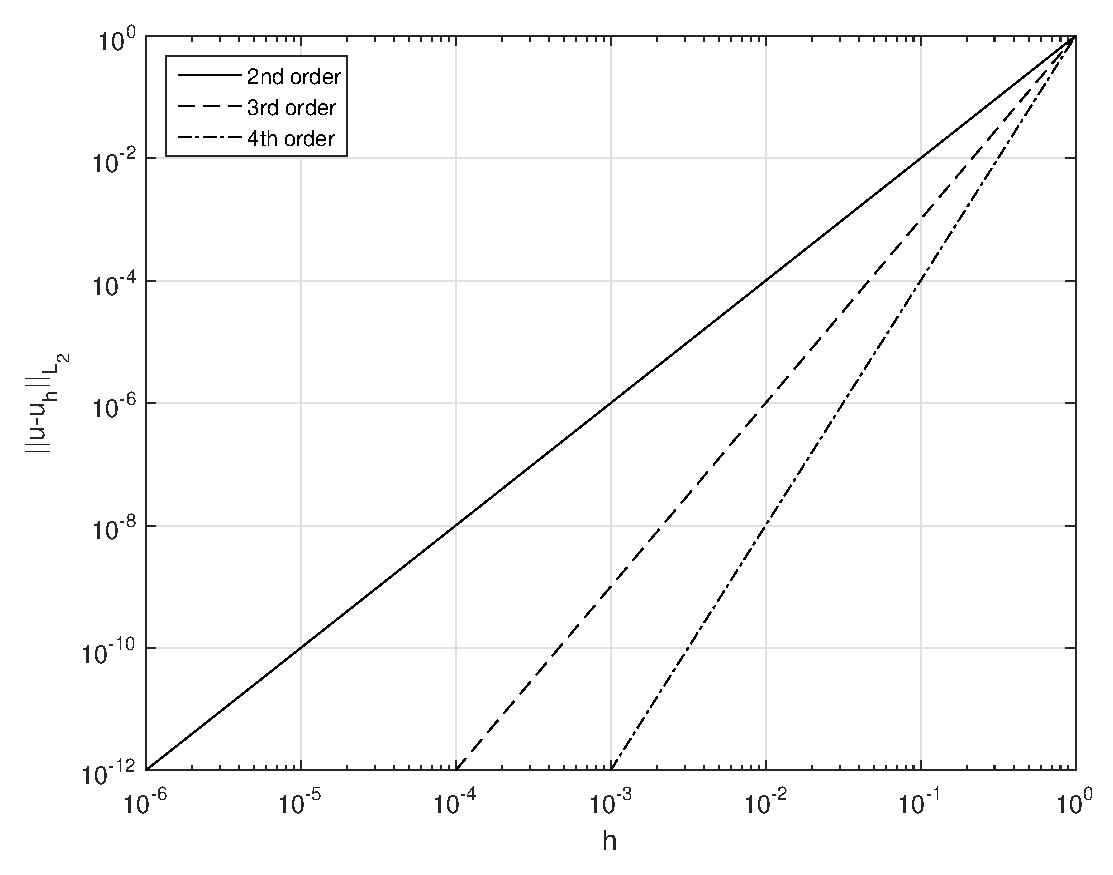
\includegraphics[width=\textwidth]{figures/sec_Sn/hconv_larger.eps}
	\end{subfigure}
	\begin{subfigure}[b]{0.495\textwidth}
		\centering
		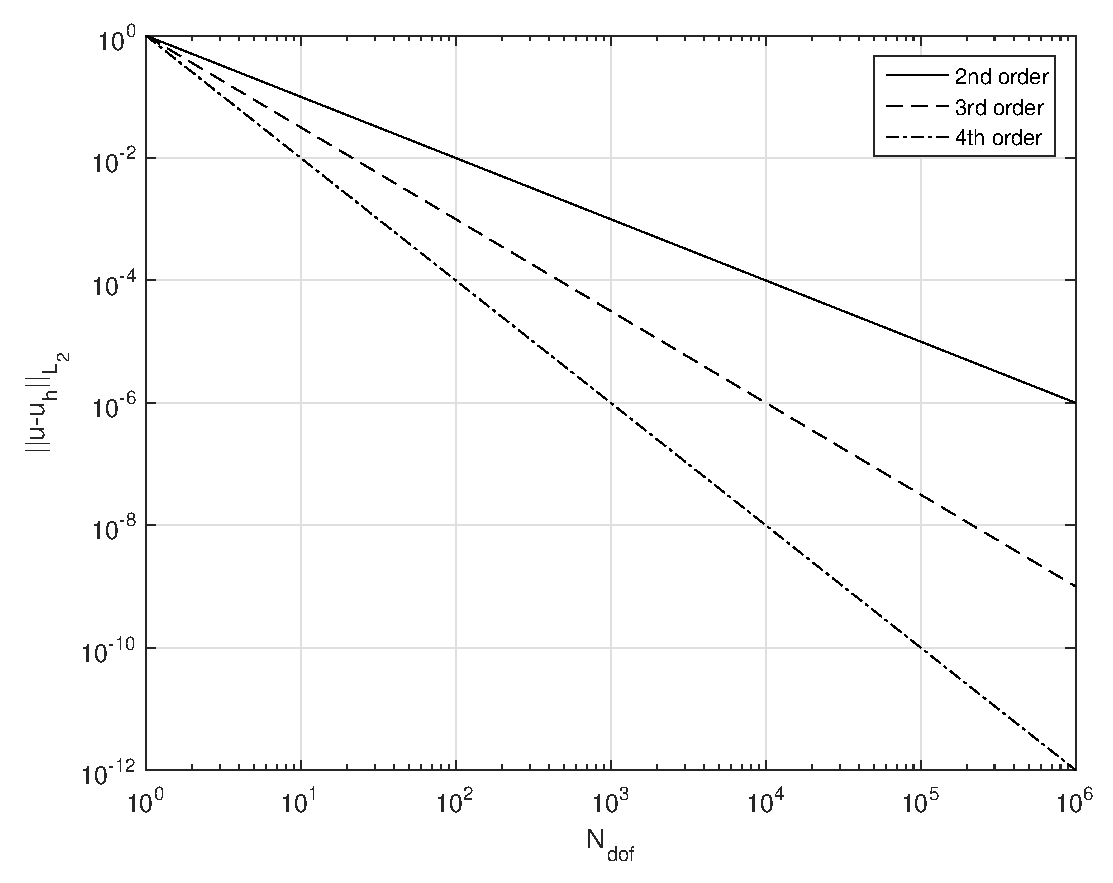
\includegraphics[width=\textwidth]{figures/sec_Sn/Nconv_larger.eps}
	\end{subfigure}
\caption[$L_2$ transport convergence rates]{blah}
\label{fig::Sn_Spatial_Convergence}
\end{figure}
%%%%%%%%%%%%%%%%%%%%%%%%%%%%%%%%%%%%%%%%%%%%%%%%%%%
%%%   SubSection - Elementary
\subsection{Elementary Matrices on an Arbitrary Spatial Cell}
\label{sec::Sn_Spatial_Matrices}

In Eq. (\ref{eq::Sn_DGFEM_trans_eq_cellK_complete}), we presented the full set of spatially-discretized equations needed to solve the angular flux solution for cell $K$ for a single angular direction. In the equation, several terms of various types arise including interaction, $\Big( \sigma  b_m , \Psi_m  \Big)_K$, streaming, $ \Big( \vec{\Omega}_m \cdot \vec{\nabla}  b_m , \Psi_m  \Big)_K$, and surface, $     \Big< \left( \vec{\Omega}_m \cdot  \vec{n} \right) \, b_m, \Psi_m  \Big>_{\partial K}$. Each of these correspond to a different elementary matrix type. We now present how to compute the mass, streaming, and surface matrices in Sections \ref{sec::Sn_Spatial_Matrices_Mass}, \ref{sec::Sn_Spatial_Matrices_Streaming}, and \ref{sec::Sn_Spatial_Matrices_Surface}, respectively.

%%%%%%%%%%%%%%%%%%%%%%%%%%%%%%%%%%%%%%%%%%%%%%%%%%%
%%%   SubSection - Mass
\subsubsection{Elementary Mass Matrices}
\label{sec::Sn_Spatial_Matrices_Mass}

In the spatially discretized equations presented in Section \ref{sec::Sn_Spatial}, there are several reaction terms that appear with the form: $\Big( \sigma  b_m , \Psi_m  \Big)_K$ for a given angular direction, $m$, and for a spatial cell, $K$. In FEM analysis these reaction terms are ubiquitously referred to as the mass matrix terms \cite{zeinkiewicz2005finite,akin1982application}. For cell $K$, we define the elementary mass matrix, ${\bf M}$, as

\begin{equation}
\label{eq::Sn_mass_matrix_analytical}
{\bf M}_K =    \int_K {\bf b}_K \, {\bf b}_K^T \, d r ,
\end{equation}

\noindent where ${\bf b}_K$ corresponds to the set of $N_K$ basis functions that have non-zero measure in cell $K$. Depending on the FEM basis functions utilized, the integrals in Eq. (\ref{eq::Sn_mass_matrix_analytical}) can be directly integrated analytically. However, if in general, the basis functions cannot be analytically integrated on an arbitrary set of cell shapes, then a numerical integration scheme becomes necessary. If we define a quadrature set, $\left\{  \vec{x}_q , w_q^{K}  \right\}_{q=1}^{N_q}$, for cell $K$, consisting of $N_q$ points, $\vec{x}_q$, and weights, $w_q^K$, then we can numerically calculate the mass matrix by the following

\begin{equation}
\label{eq::Sn_mass_matrix_numerical}
{\bf M}_K = \sum_{q = 1}^{N_q} w_{q}^K {\bf b}_K (\vec{x}_q) \, {\bf b}_K^T (\vec{x}_q)  .
\end{equation}

\noindent In this case, it is necessary that the sum of the weights of this quadrature set exactly equal the geometric measure of cell $K$. This means that $\sum_{q = 1}^{N_q} w_{q}^K$ is equal to the cell width in 1 dimension, the cell area in 2 dimensions, and the cell volume in 3 dimensions.

Since ${\bf b}_K$ consists of a column vector for the basis functions and ${\bf b}_K^{T}$ consists of a row vector, then their multiplication will obviously yield a full $(N_K \, \text{x} \, N_K)$ matrix. This matrix is written for completeness of this discussion on the mass matrix:

\begin{equation}
\label{eq::Sn_mass_matrix_array}
{\bf M}_K =   \left[
\begin{array} {ccccc}
	\int_K b_1 \, b_1  & \ldots & \int_K b_1 \, b_j  & \ldots & \int_K b_1 \, b_{N_K} \\
	\vdots  &  & \vdots  &  & \vdots \\
	\int_K b_i \, b_1  & \ldots & \int_K b_i \, b_j  & \ldots & \int_K b_i \, b_{N_K} \\
	\vdots  &  & \vdots  &  & \vdots \\
	\int_K b_{N_K} \, b_1  & \ldots & \int_K b_{N_K} \, b_j  & \ldots & \int_K b_{N_K} \, b_{N_K} \\
\end{array}
\right] ,
\end{equation}

\noindent where an individual matrix entry is of the form:

\begin{equation}
\label{eq::Sn_mass_matrix_entry}
M_{i,j,K} =  \int_K b_i \, b_j .
\end{equation}

%%%%%%%%%%%%%%%%%%%%%%%%%%%%%%%%%%%%%%%%%%%%%%%%%%%
%%%   SubSection - Streaming
\subsubsection{Elementary Streaming Matrices}
\label{sec::Sn_Spatial_Matrices_Streaming}

Next, we will consider the streaming term that has the form: $ \Big( \vec{\Omega}_m \cdot \vec{\nabla}  b_m , \Psi_m  \Big)_K$ for a given angular direction, $m$, and for a spatial cell, $K$. $\vec{\nabla} $ is the gradient operator in physical space. It has the form of $\vec{\nabla} = \left[ \frac{d}{dx} \right]$ in 1 dimension, the form of $\vec{\nabla} = \left[ \frac{\partial}{\partial x} , \frac{\partial}{\partial y} \right]$ in 2 dimensions, and the form of $\vec{\nabla} = \left[ \frac{\partial}{\partial x} , \frac{\partial}{\partial y} , \frac{\partial}{\partial z} \right]$ in 3 dimensions. Since for every cell, the streaming term is applied for all $M$ angles in the angular discretization, we define the analytical elementary streaming matrix:

\begin{equation}
\label{eq::Sn_streaming_matrix_analytical}
\vec{{\bf G}}_K =    \int_K \vec{\nabla} {\bf b}_K \, {\bf b}_K^T \, d r ,
\end{equation}

\noindent which has dimensionality $(N_K \text{x} N_K \text{x} d)$. We choose to store the elementary streaming matrix in this form and not store $M$ separate $(N_K \text{x} N_K)$ local matrices corresponding to the application of the dot product ($ \vec{\Omega}_m  \cdot \int_K  \vec{\nabla} {\bf b}_K \, {\bf b}_K^T \, d r$). Instead, we simply evaluate the dot product with the appropriate angular direction whenever necessary. This has great benefit when trying to run large transport problems when memory becomes a premium and processor operations are not our limiting bottleneck. 

Just like the elementary mass matrix, we can use the same spatial quadrature set, $\left\{  \vec{x}_q , w_q^{K}  \right\}_{q=1}^{N_q}$, for cell $K$ to numerically calculate the streaming matrix:

\begin{equation}
\label{eq::Sn_streaming_matrix_numerical}
\vec{{\bf G}}_K =    \sum_{q = 1}^{N_q} w_{q}^K \vec{\nabla} {\bf b}_K (\vec{x}_q) \, {\bf b}_K^T (\vec{x}_q) .
\end{equation}

\noindent In this case, this local cell-wise streaming matrix has the full matrix form:

\begin{equation}
\label{eq::Sn_streaming_matrix_array}
\vec{{\bf G}}_K =   \left[
\begin{array} {ccccc}
	\int_K \vec{\nabla}b_1 \, b_1  & \ldots & \int_K \vec{\nabla}b_1 \, b_j  & \ldots & \int_K \vec{\nabla}b_1 \, b_{N_K} \\
	\vdots  &  & \vdots  &  & \vdots \\
	\int_K \vec{\nabla} b_i \, b_1  & \ldots & \int_K \vec{\nabla}b_i \, b_j  & \ldots & \int_K \vec{\nabla}b_i \, b_{N_K} \\
	\vdots  &  & \vdots  &  & \vdots \\
	\int_K \vec{\nabla} b_{N_K} \, b_1  & \ldots & \int_K \vec{\nabla} b_{N_K} \, b_j  & \ldots & \int_K \vec{\nabla} b_{N_K} \, b_{N_K} \\
\end{array}
\right] ,
\end{equation}

\noindent where an individual matrix entry is of the form:

\begin{equation}
\label{eq::Sn_streaming_matrix_entry}
\vec{G}_{i,j,K} =  \int_K \vec{\nabla}b_i \, b_j .
\end{equation}

%%%%%%%%%%%%%%%%%%%%%%%%%%%%%%%%%%%%%%%%%%%%%%%%%%%
%%%   SubSection - Surface
\subsubsection{Elementary Surface Matrices}
\label{sec::Sn_Spatial_Matrices_Surface}

Finally, the last terms to consider of the discretized transport equation are those found on the faces of the cell boundary: $  \vec{\Omega}_m \cdot  \Big<  \vec{n} \, b_m, \Psi_m  \Big>_{\partial K}$. These terms are analagous to the cell mass matrix but are computed on the cell boundary with dimensionality $(d-1)$. Analyzing a single face, $f$, in cell $K$, the analytical surface matrix is of the form,

\begin{equation}
\label{eq::Sn_surface_matrix_analytical}
\vec{{\bf F}}_{f,K}  =    \int_f \vec{n} (\vec{r}) \, {\bf b}_K \, {\bf b}_K^T \, d s ,
\end{equation}

\noindent where we allow the outward surface normal, $\vec{n}$, to vary along the cell face. For 1D problems as well as 2D problems with colinear cell faces (no curvature), the outward normals would be constant along the entire face. However, there are many cases where 3D mesh cells would not have coplanar vertices along a face. Then, the outward normal would not be constant along the face and would need to be taken into account during integration procedures. A simple example of non-coplanar face vertices would be an orthogonal hexahedral cell that has its vertices undergo a randomized displacement.

With the analytical form of the surface matrices defined in Eq. (\ref{eq::Sn_surface_matrix_analytical}), we can see that they have dimensionality, $(N_K \text{x} N_K \text{x} d)$. This is the same dimensionality as the cell streaming term. However, it is possible to reduce the dimensionality of the surface matrices if it is desired to reduce the memory footprint. There are some basis sets where all but $N_b^{f,K}$ basis functions are zero along face $f$. If we also restrict the mesh cell faces of our transport problems to have colinear (in 2D) or coplanar (in 3D) vertices so that the outward normal is constant along a face $f$, then we can define the surface matrix as $\int_f {\bf b}_K \, {\bf b}_K^T \, d s$. For these basis sets with $N_b^{f,K}$ non-zero face values on colinear/coplanar face $f$, the surface matrix has reduced dimensionality of $(N_b^{f,K} \text{x} N_b^{f,K})$.

Just like the cell mass and streaming matrices, it is possible that the basis functions cannot be integrated analytically. Analogous to the cell-wise quadrature, we can define a quadrature set for face $f$: $\left\{  \vec{x}_q , w_q^{f}  \right\}_{q=1}^{N_q^f}$. This quadrature set is not specific for just one of the cells that face $f$ separates. If the quadrature set can exactly integrate the basis functions of both cells $K$ and $K'$ (as defined by Figure \ref{fig::Sn_two_ref_cells}), then only 1 quadrature set needs to be defined for both cells. Using this quadrature set, we can numerically calculate the surface matrix for face $f$ along cell $K$:

\begin{equation}
\label{eq::Sn_surface_matrix_numerical}
\vec{{\bf F}}_{f,K} =    \sum_{q = 1}^{N_q^f} w_{q}^f \vec{n} (\vec{x}_q) \, {\bf b}_K (\vec{x}_q) \, {\bf b}_K^T (\vec{x}_q) .
\end{equation}

\noindent Similar to the cell-wise spatial quadrature sets, the sum of the weights of these face-wise quadrature sets needs to exactly equal the geometric measure of face $f$. This means that $\sum_{q = 1}^{N_q^f} w_{q}^f$ is equal to 1.0 in 1 dimension, the length of the face edge in 2 dimensions and the face area in 3 dimensions. 

Using the same notation as the cell-wise mass and streaming matrices, the local face-wise surface matrix for face $f$ has the full matrix form,

\begin{equation}
\label{eq::Sn_surface_matrix_array}
\vec{{\bf F}}_{f,K} =   \left[
\begin{array} {ccccc}
	\int_f \vec{n} \, b_1 \, b_1  & \ldots & \int_f \vec{n} \, b_1 \, b_j  & \ldots & \int_f \vec{n} \, b_1 \, b_{N_K} \\
	\vdots  &  & \vdots  &  & \vdots \\
	\int_f \vec{n} \,  b_i \, b_1  & \ldots & \int_f \vec{n} \, b_i \, b_j  & \ldots & \int_f \vec{n} \, b_i \, b_{N_K} \\
	\vdots  &  & \vdots  &  & \vdots \\
	\int_f \vec{n} \,  b_{N_K} \, b_1  & \ldots & \int_f \vec{n} \,  b_{N_K} \, b_j  & \ldots & \int_f \vec{n} \,  b_{N_K} \, b_{N_K} \\
\end{array}
\right] ,
\end{equation}

\noindent where an individual matrix entry is of the form:

\begin{equation}
\label{eq::Sn_surface_matrix_entry}
\vec{{ F}}_{i,j,f,K} =  \int_f \vec{n} \, b_i \, b_j .
\end{equation}

%%%%%%%%%%%%%%%%%%%%%%%%%%%%%%%%%%%%%%%%%%%%%%%%%%%
%%%   Section - Solution Procedures
\section{Solution Procedures}
\label{sec::Sn_Solution}

To this point, we have properly described the procedures to discretize the transport problem in energy, angle, and space. Combining the results of Sections \ref{sec::Sn_MG}, \ref{sec::Sn_Angle}, and \ref{sec::Sn_Spatial}, we write the fully-discretized DGFEM multigroup $S_N$ equations for an element $K$, where the test function $b_{m,g}$ for a single direction and energy group is now used:

\begin{equation}
\label{eq::Sn_DGFEM_trans_eq_cellK_bmg_complete}
\begin{aligned}
-  \Big( \vec{\Omega}_m \cdot  & \vec{\nabla} b_{m,g}, \Psi_{m,g} \Big)_{K}   + \Big(  \sigma_{t,g} b_{m,g} ,   \Psi_{m,g} \Big)_{K} +  \Big< ( \vec{\Omega}_m \cdot \vec{n} ) \, b_{m,g}, {\Psi}_{m,g}^{-}  \Big>_{\partial K^+}  \\
  + & \Big< ( \vec{\Omega}_m \cdot \vec{n} ) \, b_{m,g}, {\Psi}_{m,g}^{+}  \Big>_{\partial K^- \backslash \partial \mathcal{D}}  + \Big< ( \vec{\Omega}_m \cdot \vec{n} ) \, b_{m,g}, {\Psi}^{-}_{m',g}  \Big>_{\partial K^- \cap \partial \mathcal{D}^r}  \\
= & \sum\displaylimits_{g'=1}^G \sum_{p=0}^{N_P} \frac{2p + 1}{4 \pi} \sum_{n=-p}^{p}   Y_{p,n} (  \vec{\Omega}_m )  \Big( \sigma_{s,p}^{g' \rightarrow g} \, b_{m,g},  \Phi_{p,n,g'} \Big)_{K}  \\
+ & \left(  b_{m,g} ,   Q_{m,g} \right)_{K} - \Big< ( \vec{\Omega}_m \cdot \vec{n} ) \, b_{m,g}, {\Psi}_{m,g}^{inc}  \Big>_{\partial K^- \cap \partial \mathcal{D}^d}
\end{aligned} .
\end{equation} 

\noindent All of the notations used in Eq. (\ref{eq::Sn_DGFEM_trans_eq_cellK_bmg_complete}) remain unchanged from Section \ref{sec::Sn_Spatial}.

We now spend the remainder of this chapter discussing various methodologies to efficiently solve the tightly-coupled system of equations composing our transport problem. Section \ref{sec::Sn_Solution_Iterative} details the iterative procedures used to solve the transport problem in energy and angle, and Section \ref{sec::Sn_Solution_Spatial} then describes how we solve the spatial portion of the problem for a single energy/angle iteration.

%%%%%%%%%%%%%%%%%%%%%%%%%%%%%%%%%%%%%%%%%%%%%%%%%%%
%%%   SubSection - Iterative Procedures
\subsection{Angle and Energy Iteration Procedures}
\label{sec::Sn_Solution_Iterative}

The fully discretized transport equation has an angular flux solution, ${\bf \Psi}$, with dimensionality of $(G \text{x} M \text{x} N_{dof})$. The angular flux moments, ${\bf \Phi}$, have dimensionality of $(G \text{x} N_{mom} \text{x} N_{dof})$. Depending on the necessary fidelity of the problem, the full phase-space of the solution can become extremely large to solve. We can have {\em billions} of total unknowns to solve for if we simply have $N_{dof} \approx O(10^6)$, $M \approx O(10^2)$, and $G \approx O(10^1)$. These orders of number of unknowns in space, angle, and energy are of reasonable size for 3D transport problems.

In theory, if we had the computer memory, we could construct a left-hand-side matrix of dimensionality $(G \text{x} M \text{x} N_{dof})$x$(G \text{x} M \text{x} N_{dof})$ with a corresponding right-hand-side vector of dimensionality $(G \text{x} M \text{x} N_{dof})$x1, we could then directly solve for the full phase-space angular flux solution at once. However, because the dimensional space of the unknowns can rapidly grow and become too large for hardware memory, transport problems have traditionally been solved iteratively. We now detail the procedures that we will employ to iteratively obtain the phase-space solution in energy and angle.

Because the only coupling that arises between the set of multigroup $S_N$ equations is between the energy groups in the scattering source, our iterative procedures principally lie in the energy domain. 

\begin{figure}
\centering
	\begin{subfigure}[b]{0.58\textwidth}
		\centering
		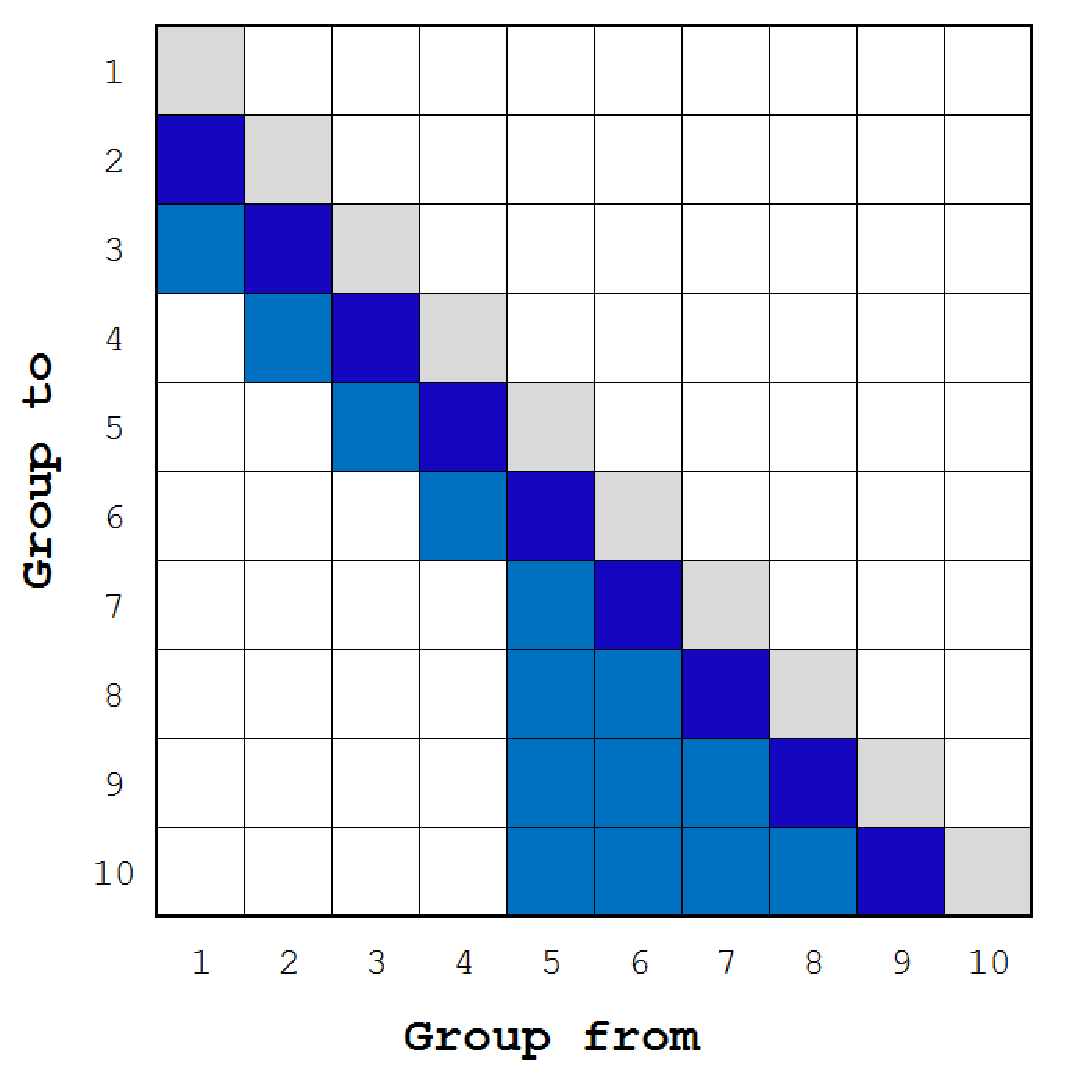
\includegraphics[width=\textwidth]{figures/sec_Sn/scattering_matrix_NO_upscattering.eps}
		\vspace{4mm}
	\end{subfigure}
	\hfill
	\begin{subfigure}[b]{0.58\textwidth}
		\centering
		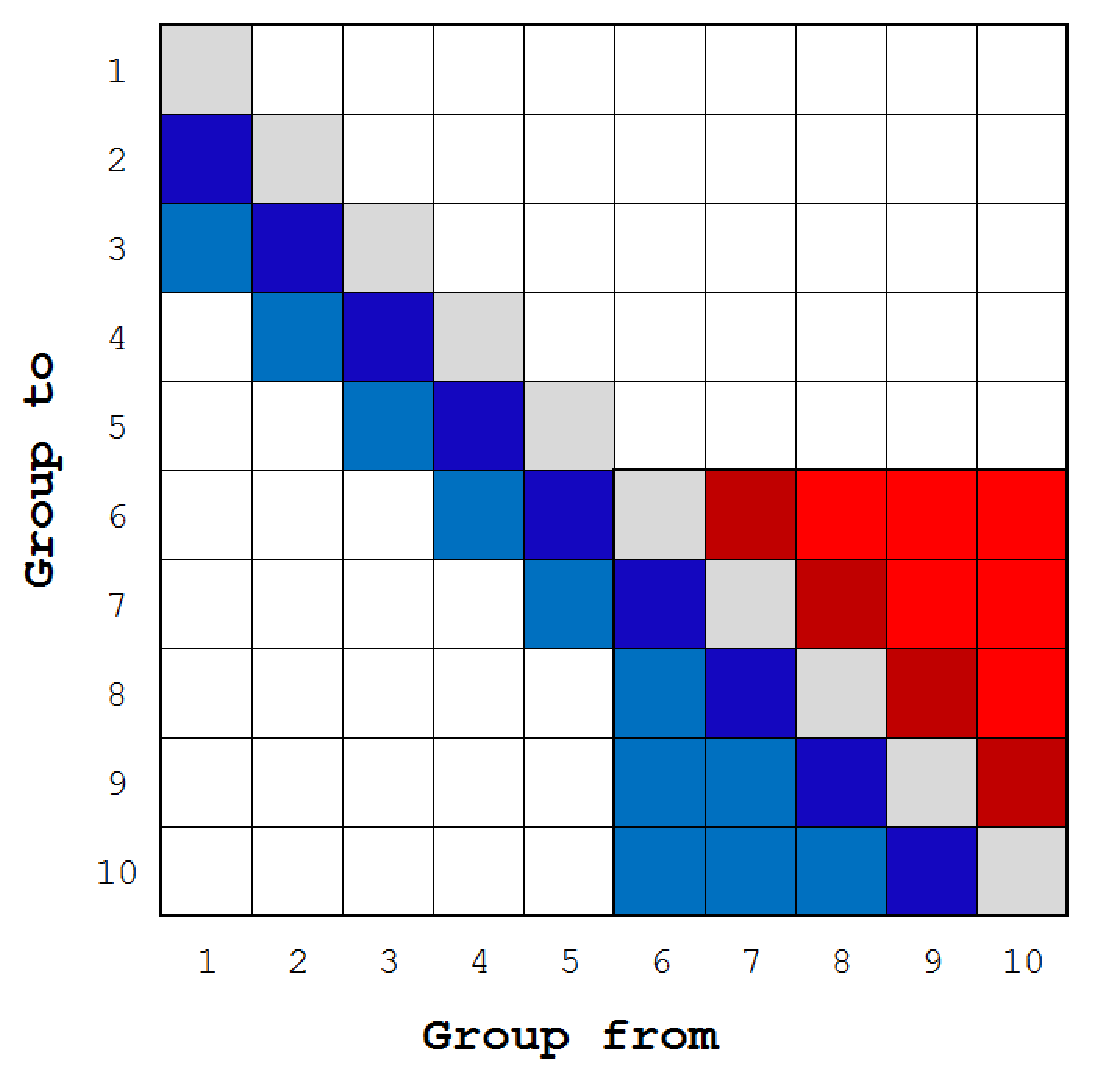
\includegraphics[width=\textwidth]{figures/sec_Sn/scattering_matrix_w_upscattering.eps}
	\end{subfigure}
\caption[Scattering matrices with and without upscattering]{Scattering matrices (top) without and (bottom) with upscattering. The gray corresponds to within-group scattering; the blue corresponds to down-scattering in energy; and the red corresponds to up-scattering in energy.}
\label{fig::Sn_Solution_Iterative_scattmatrix}
\end{figure}

\begin{equation}
\label{eq::Sn_full_sol_ops}
\begin{aligned}
{\bf L} {\bf \Psi} - {\bf M} {\bf \Sigma} {\bf \Phi}  =    {\bf Q} \\
{\bf \Phi} =  {\bf D} {\bf \Psi}
\end{aligned}
\end{equation}

\noindent where ${\bf L}$ is the fully-discretized loss operator which consists of total interaction and streaming terms, ${\bf M}$ is the moment-to-discrete operator of the angular discretization, ${\bf D}$ is the discrete-to-moment operator of the angular discretization, ${\bf \Sigma}$ is the scattering operator of the multigroup and angular discretizations, and ${\bf Q}$ is the full phase-space distributed source. In this case, the source contains contributions from boundary and domain sources, fission sources, and scattering sources from outside the group set into the group set of interest.



\begin{equation}
\label{eq::Sn_full_sol_moments_only}
\left( {\bf I} -{\bf T} \right) {\bf \Phi} =  {\bf D} {\bf L}^{-1}  {\bf Q} 
\end{equation}

\noindent where we define,

\begin{equation}
\label{eq::Sn_trans_op_T}
{\bf T} \equiv {\bf D} {\bf L}^{-1}{\bf M} {\bf \Sigma} ,
\end{equation}

\noindent for further brevity.



%%%%%%%%%%%%%%%%%%%%%%%%%%%%%%%%%%%%%%%%%%%%%%%%%%%
%%%   SubSubSection - Source Iteration
\subsubsection{Source Iteration}
\label{sec::Sn_Solution_Iterative_SI}

One simple method to invert $({\bf I} - {\bf T})$ of Eq. (\ref{eq::Sn_full_sol_moments_only}) is the {\em source iteration} technique, also known as {\em richardson iteration}. If we isolate a single group set, $gs$, then the 

\begin{equation}
\label{eq::Sn_pre_si_iter}
{\bf L}_{gs} {\bf \Psi}_{gs}^{(\ell+1)} =    {\bf M}_{gs} {\bf \Sigma}_{gs} {\bf \Phi}_{gs}^{(\ell)} +  {\bf Q}_{gs} 
\end{equation}

\begin{equation}
\label{eq::Sn_si_iter}
\begin{aligned}
 {\bf \Psi}_{gs}^{(\ell+1)} = {\bf L}_{gs}^{-1} \left(  {\bf M}_{gs} {\bf \Sigma}_{gs} {\bf \Phi}_{gs}^{(\ell)} +  {\bf Q}_{gs} \right) \\
{\bf \Phi}_{gs}^{(\ell+1)} =  {\bf D}_{gs} {\bf \Psi}_{gs}^{(\ell+1)}
\end{aligned}
\end{equation}

%%%%%%%%%%%%%%%%%%%%%%%%%%%%%%%%%%%%%%%%%%%%%%%%%%%
%%%   SubSubSection - Source Iteration
\subsubsection{Krylov Subspace Methods}
\label{sec::Sn_Solution_Iterative_GMRES}

Source iteration is not the only iterative technique that can be employed to invert $({\bf I} - {\bf T})$ for a given group set. In the last 20 years, krylov subspace methods have been applied to the discretized transport equation \cite{oliveira1998preconditioned,guthrie1999gmres,patton2002application}. Because $({\bf I} - {\bf T})$ is not symmetric, we want to only use krylov methods that can solve non-symmetric matrices. The two krylov subspace methods that we would naturally want to employ are GMRES and BiCGSTAB \cite{saad1986gmres,saad2003iterative}. We will not describe the implementations of these methods here for brevity. However, we will state that most of the computational machinery required to perform richardson iterations can also be used for these krylov methods. The only modifications/extensions that are needed are summarized in the following list.

\begin{enumerate}
\item Construction of the right-hand-side: ${\bf b} = {\bf D} {\bf L}^{-1} {\bf Q}$. From this equation, it is obvious that we need just one initial transport sweep to properly build this right-hand-side.
\item The operation of the matrix $({\bf I} - {\bf T})$ on a krylov vector, $\nu$. This can easily be accomplished with the same machinery as richardson iteration by simply subtracting the original flux moment vector by the updated moments after one transport sweep.
\item Modify the calculation of the convergence criterion so that the norm of the iteration residual, normalized by the right-hand-side, is smaller than some prescribed tolerance:
$\frac{||{\bf b} - ({\bf I} - {\bf T}) {\bf x} ||_2}{||{\bf b}||_2} < \text{tol}$.
\end{enumerate}

Combined with the appropriate linear algebra operations, these three small alterations are all that are required to properly utilize the krlov solver for the transport equation. It is not immediately obvious how one would would precondition the krylov iterations in the context of transport sweeping. However, just like the richardson iteration scheme, we will provide the implementation of DSA preconditioning for krylov in Chapter \ref{sec::DSA}.

%%%%%%%%%%%%%%%%%%%%%%%%%%%%%%%%%%%%%%%%%%%%%%%%%%%
%%%   SubSection - Spatial Solution Procedures
\subsection{Spatial Solution Procedures}
\label{sec::Sn_Solution_Spatial}

Section \ref{sec::Sn_Solution_Iterative} presented the methodology that we will employ to iteratively converge our transport solutions in energy and angle (flux moments). Both richardson iteration and the krylov methods were presented as methods that can invert the $({\bf I} - {\bf T})$ operator. In both of these iterative methods, the common operation of interest is the inversion of the loss operator (${\bf L}$). There are different techniques that could be used to perform this operation, including several matrix-dependent and matrix-free methodologies. 

For this work, the loss operator inversion on some unstructured mesh, $\mathbb{T}_h$, will be performed by use of the full-domain transport sweep as outlined next in Section \ref{sec::Sn_Solution_Spatial_Sweeping}. We will generate our 2D and 3D polytope meshes by two different methods: 1) Voronoi mesh generation in Section \ref{sec::Sn_Solution_Spatial_Voronoi} and 2) adaptive mesh refinement in Section \ref{sec::Sn_Solution_Spatial_AMR}.

%%%%%%%%%%%%%%%%%%%%%%%%%%%%%%%%%%%%%%%%%%%%%%%%%%%
%%%   SubSubSection - Transport Sweeping
\subsubsection{Transport Sweeping}
\label{sec::Sn_Solution_Spatial_Sweeping}

The full-domain transport sweep is a beneficial matrix-free scheme because of the following:

\begin{itemize}
\item The number of sweep iterations does not grow with increasing problem size or processor counts. This is in contrast with partial-domain sweeping like {\em parallel block jacobi} (PBJ) \cite{zerr2011solution}.
\item The iterative solver does not need to build any matrices explicitly but only requires the action of ${\bf L}^{-1}$.
\item Does not require the formation of $M$ separate matrices for each of the angular directions (for 1 energy group). This is both memory and computationaly intensive for any problems of appreciable size.
\item The matrix-vector operations on a single element within a transport sweep can be efficiently performed depending on the group set structure and the angle aggregation as outlined in Section \ref{sec::Sn_Solution_Iterative}.
\item The matrix-free transport sweep favors higher-order DGFEM schemes since they will yield more processor work per element with less memory caching (which is the current bottleneck with massively-parallel calculations).
\end{itemize}

\begin{figure}
\centering
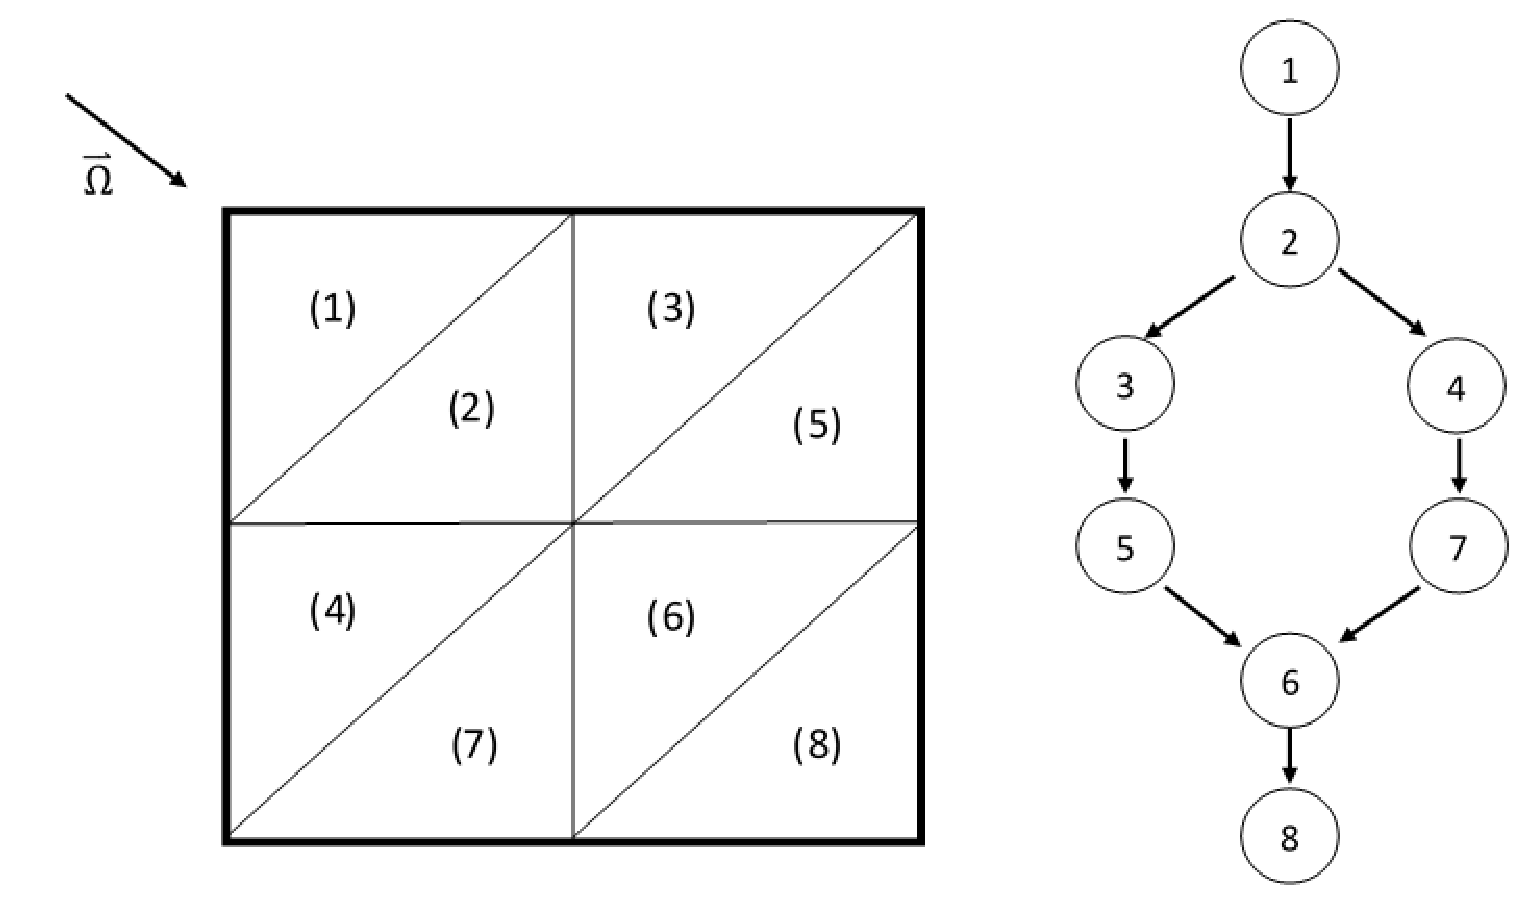
\includegraphics[width=0.75\textwidth]{figures/sec_Sn/triangle_graph_nocycle.eps}
\caption[blah]{blah.}
\label{fig::Sn_Solution_Spatial_Sweeping_sweepNOcycle}
\end{figure}

\begin{figure}
\centering
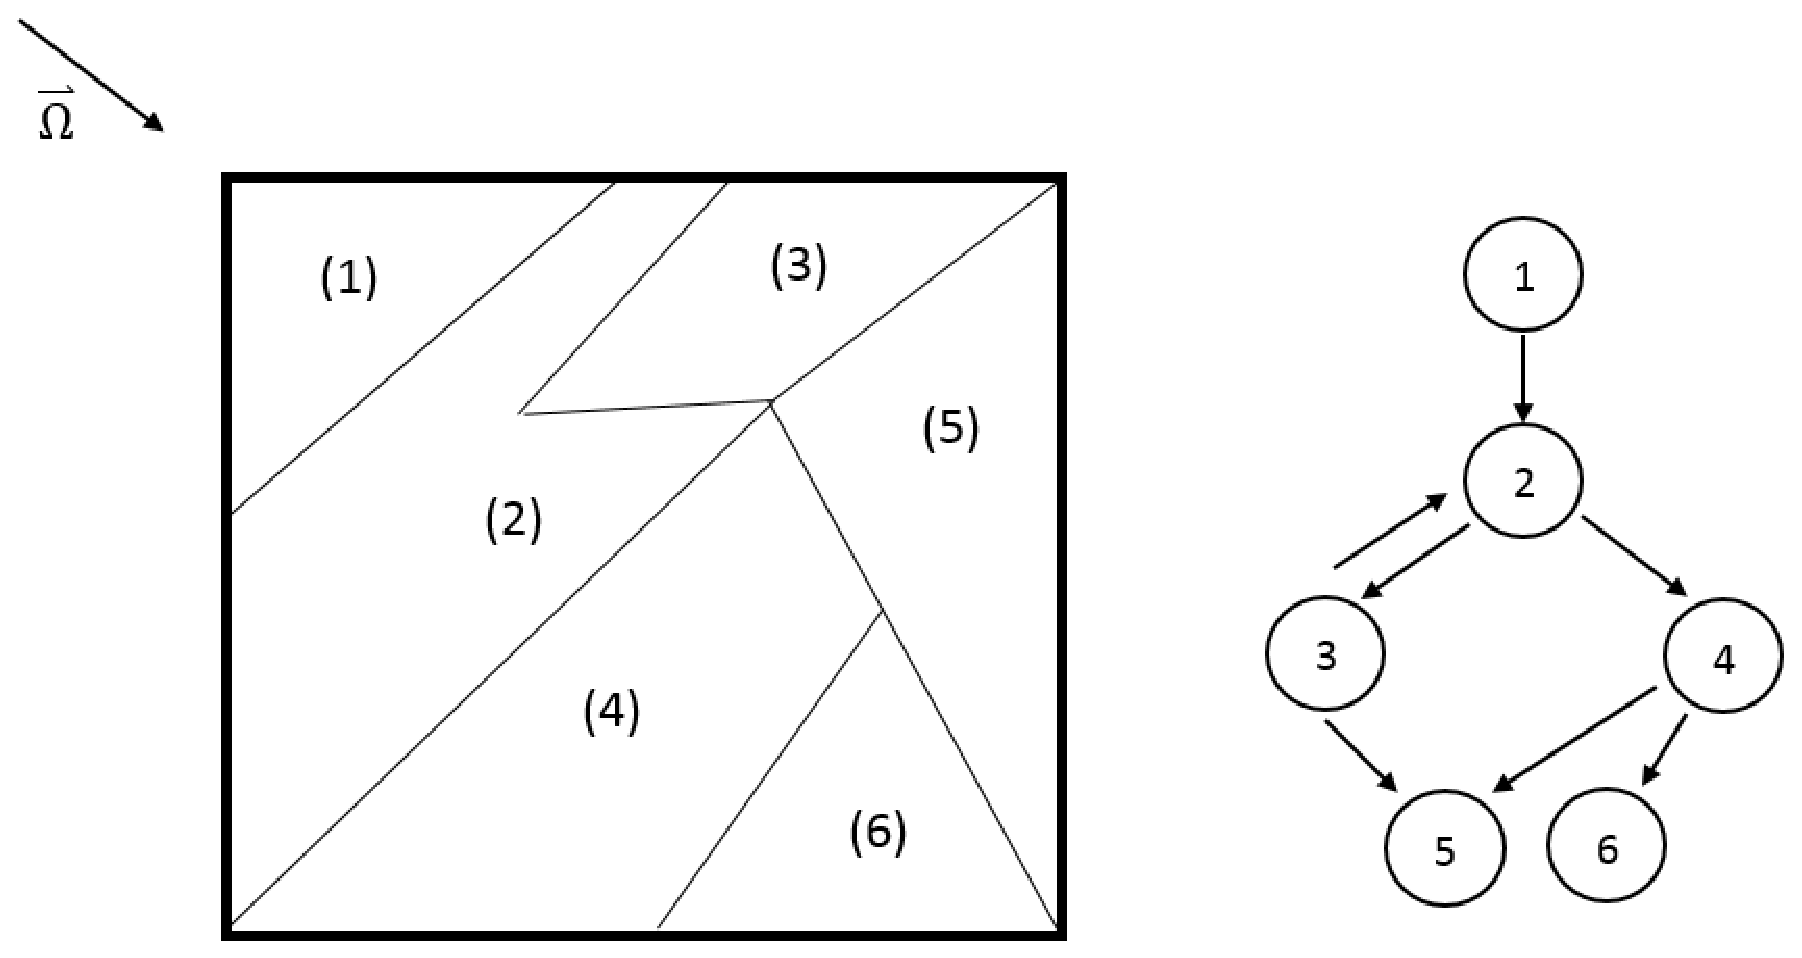
\includegraphics[width=0.75\textwidth]{figures/sec_Sn/graph_with_cycling.eps}
\caption[blah]{blah.}
\label{fig::Sn_Solution_Spatial_Sweeping_sweepWcycle}
\end{figure}

%%%%%%%%%%%%%%%%%%%%%%%%%%%%%%%%%%%%%%%%%%%%%%%%%%%
%%%   SubSubSection - Voronoi
\subsubsection{Polytope Grids Formed from Voronoi Mesh Generation}
\label{sec::Sn_Solution_Spatial_Voronoi}



%%%%%%%%%%%%%%%%%%%%%%%%%%%%%%%%%%%%%%%%%%%%%%%%%%%
%%%   SubSubSection - AMR
\subsubsection{Spatial Adaptive Mesh Refinement}
\label{sec::Sn_Solution_Spatial_AMR}



\begin{equation}
\label{eq::Sn_AMR_jump_err_est}
\eta_K^r = \int\displaylimits_{\partial K} [\![ \Phi^r ]\!]^2 d \, s = \int\displaylimits_{\partial K} \left(  \sum_m w_m [\![ \Psi_m^r ]\!]  \right)^2
\end{equation}

\noindent where $[\![ \cdot ]\!]$ is the jump operator along a face defined as,

\begin{equation}
\label{eq::Sn_AMR_jump_def}
[\![ \Phi (\vec{r}) ]\!] = \Phi^+ (\vec{r}) - \Phi^- (\vec{r}),
\end{equation}

\noindent and the terms,$\Phi^+ (\vec{r})$ and $\Phi^- (\vec{r})$, are subject to the trace:

\begin{equation}
\label{eq::Sn_AMR_jump_trace}
\Phi^{\pm} (\vec{r})  = \lim\displaylimits_{s \rightarrow 0^{\pm}} \Phi (\vec{r} + s \vec{n}).
\end{equation}

\noindent In this case, the outward normal, $\vec{n}$, is determined with respect to the element $K$ along its boundary, $\partial K$. With this trace, $\Phi^- (\vec{r})$ always corresponds to the solution within cell $K$. Investigating face $f$ of cell $K$, the across-face solution, $\Phi^+ (\vec{r})$, is dependent on the boundary type of face $f$. The across-face solutions can be succinctly written:

\begin{equation}
\label{eq::Sn_AMR_across_face_vals}
\Phi^+ (\vec{r}) = 
\begin{cases}
\lim\displaylimits_{s \rightarrow 0^{+}} \Phi (\vec{r} + s \vec{n}) & \vec{r} \notin \partial \mathcal{D} \\
\sum\displaylimits_{\vec{\Omega}_m \cdot \vec{n} > 0}  \Psi_m^- (\vec{r}) + \sum\displaylimits_{\vec{\Omega}_m \cdot \vec{n} < 0} \Psi_{m}^{inc} (\vec{r}) & \vec{r} \in \partial \mathcal{D}^d \\
\Phi^- (\vec{r}) & \vec{r} \in \partial \mathcal{D}^r
\end{cases}.
\end{equation}

\noindent From Eq. (\ref{eq::Sn_AMR_across_face_vals}), the across-face solutions for interior faces, incident boundaries and reflecting boundaries have different meanings. For an interior face $f$ ($\vec{r} \notin \partial \mathcal{D}$), the across-face solution comes from the cell $K'$ (as defined by Figure \ref{fig::Sn_two_ref_cells}). For incident boundaries ($\vec{r} \in \partial \mathcal{D}^d$), the across-face solution is a combination of integrals of the outgoing ($\Psi_m^-$) and incident boundary fluxes ($\Psi_m^{inc}$). Finally, for reflecting boundaries ($\vec{r} \in \partial \mathcal{D}^r$), the across-face solutions are simply the within-cell solutions. Therefore, the solution jump is exactly zero for all reflecting boundaries and yields no contribution to the error estimate.

With the error estimates defined for all cells $K \in \mathbb{T}_h^r$ for refinement level $r$, a criterion is needed to determine which cells should be refined. For this work, we choose to employ

\begin{equation}
\label{eq::Sn_AMR_err_crit}
\eta_K^r \geq \alpha \max\displaylimits_{K' \in \mathbb{T}_h^r} \left(  \eta_{K'}^{r} \right),
\end{equation}

\noindent where $\alpha$ is a user-defined value $(0,1)$. This refinement criterion has a simple meaning. If, for example, $\alpha = 0.2$, then a cell will be refined if its error estimate is greater than 20\% of the cell with the largest error estimate. This does not necessarily mean that 80\% of the mesh cells will be refined at level $r$. Instead, the criterion simply states that any cell above a particular threshold will be refined. This means that it is theoretically possible for the extreme cases of 1 or all cells being refined at a particular refinement cycle. The first extreme case could arise with a single spatial cell having a strong solution discontinuity stemming from a strong localized source. The second extreme case could arise when the intercell solution jumps are about equivalent stemming from an incredibly smooth discretized solution at that particular refinement cycle. We could also enforce a uniform refinement of all the spatial cells by setting $\alpha=0$.


%%%%%%%%%%%%%%%%%%%%%%%%%%%%%%%%%%%%%%%%%%%%%%%%%%%
%%%   Section - Conclusions
\section{Conclusions}
\label{sec::Sn_Conclusions}

In this chapter, we have presented the tightly-coupled system of equations that comprise the DGFEM $S_N$ transport equation. We began with the fully-continuous transport equation presented in Section \ref{sec::Sn_neut} and then discretized it in energy, angle and space in Sections \ref{sec::Sn_MG}, \ref{sec::Sn_Angle}, and \ref{sec::Sn_Spatial}, respectively. Appropriate boundary conditions were presented in Section \ref{sec::Sn_BC}. For this work, we will only utilize incoming-incident and reflecting boundary conditions and not use any further albedo terms. We finished this chapter in Section \ref{sec::Sn_Solution} by describing the procedures that will be utilized to solve our system of equations.

